% Inicio del preámbiulo
\documentclass[letterpaper,12pt]{article} %Modifica el tipo de documento y el tamaño de la letra.
\usepackage[utf8]{inputenc}
\usepackage[T1]{fontenc}
\usepackage[shortlabels]{enumitem}
\usepackage[spanish,mexico]{babel} 
\usepackage{amsmath,amssymb,amsfonts,latexsym,cancel}
\usepackage{hyperref}
\usepackage{wrapfig}
\usepackage[rflt]{floatflt}
\usepackage[pdftex]{graphicx}
\usepackage{fancyhdr}
\usepackage{bookmark}
\usepackage{float}
\usepackage{longtable,multirow,booktabs}
\usepackage{cite}
\usepackage{wrapfig}
\usepackage{multicol}
\usepackage{caption}
\usepackage[]{sidecap}
\usepackage{adjustbox}
\usepackage{parskip}
\usepackage{enumitem}
\usepackage{tikz}
\usepackage{lipsum}
\usepackage[]{xcolor}
\usepackage{multicol}
\usepackage{listings}
\usepackage{tabularx}
\usepackage{booktabs}
\usepackage{array}
\setcounter{secnumdepth}{5}
\setcounter{tocdepth}{5}
\usepackage{graphicx}
\usepackage{subcaption}
\usepackage{pgfplots}
\pgfplotsset{compat=1.18}
\usepgfplotslibrary{groupplots,colormaps}
\usepackage{tcolorbox}
%Fin de Préambulo


% Variables del documento
\newcommand{\myMateria}{Simulación}
\newcommand{\myGrupo}{20}
\newcommand{\myUnidad}{}
\newcommand{\mySemester}{2025-2}
\newcommand{\MyReport}{Proyecto}
\newcommand{\myDate}{29 de enero 2026}
\newcommand{\myName}{{Gael Ruiz Ñurinda}{\\Anthony Segura Paniagua}{\\Sebastián Castillo Monestel}{\\Saúl Pacheco Cubillo}}
\newcommand{\myTeacher}{Eddy Ramírez Jiménez}


%Inicio formato de Página.
\textheight = 21cm %Medidas de la  página
\textwidth = 18cm  %Medidas de la página
\topmargin = -2cm  %Medidas de la página    
\oddsidemargin = -0.8cm %Medidas de la página
\pagestyle{fancy} %Diseño de la página

\fancyhf{}
\lhead{} %%LeftHead
\chead{
\includegraphics[ height=1cm]{Imágenes/logo-itcr.png}} %%CenterHead
%\lfoot{USM}
% \rhead{Unidad \myUnidad} %%RightHead

\setlength{\columnsep}{4mm}%Comandos para el formato de la página.
%\setlength{\parindent}{4em}%Sangría al comenzar un nuevo párrafo.
\setlength{\parindent}{0.5in}
%\setlength{\parindent}{4em}%Sangría al comenzar un nuevo párrafo.
\setlength{\parskip}{1em}%Distancia entre párrafos.
\renewcommand{\baselinestretch}{1.0}% Espacio entre línea y línea o interlineado.
\setlength{\headheight}{33pt}
\fancyfoot[C,CO]{\thepage} %Logo de LaTeX y pie de página.
%Fin formato de Página


%Aquí inicia el documento.
\begin{document}

% Inserta la portada
\thispagestyle{empty}

\begin{figure}[ht]
    \minipage{0.7\textwidth}
        
\includegraphics[width=5cm]{Imágenes/logo-itcr.png}
        \label{logoITCR}
    \endminipage
\end{figure}

\vspace{0.1cm}

\begin{center}
    {\Large \textbf{INSTITUTO TECNOLÓGICO DE COSTA RICA} \par}
	{\scshape\Large Ingeniería en Computación \par}
    \vspace{0.75cm}
    {\Large \textbf{\myMateria} \par}

    {\Large Grupo: \myGrupo \par}
    \vspace{0.95cm}
    
    {\LARGE\bfseries \MyReport\\Simulación para Sistema de Colas\par}
    \vspace{0.95cm}
    
    {\scshape\Large Fecha de entrega: \myDate \par}  
    \vspace{0.95cm}
    
    {\LARGE \textbf{Profesor:}} \\\vspace{0.1cm}
    {\large \myTeacher}
    
    \vspace{0.5cm}  
    
    {\LARGE \textbf{Estudiantes:}} \\\vspace{0.3cm}
    {\normalsize \myName}

    \vfill
\end{center}

\newpage
\tableofcontents
\newpage

% Insertar el contenido
\section{Análisis de distribuciones}

% Cajas
\subsection{Servidor cajas}
\subsubsection*{1.1.1.\hspace{0.5em} Análisis de frecuencias}
\begin{figure}[H]
    \centering
    \begin{subfigure}{0.55\textwidth}
        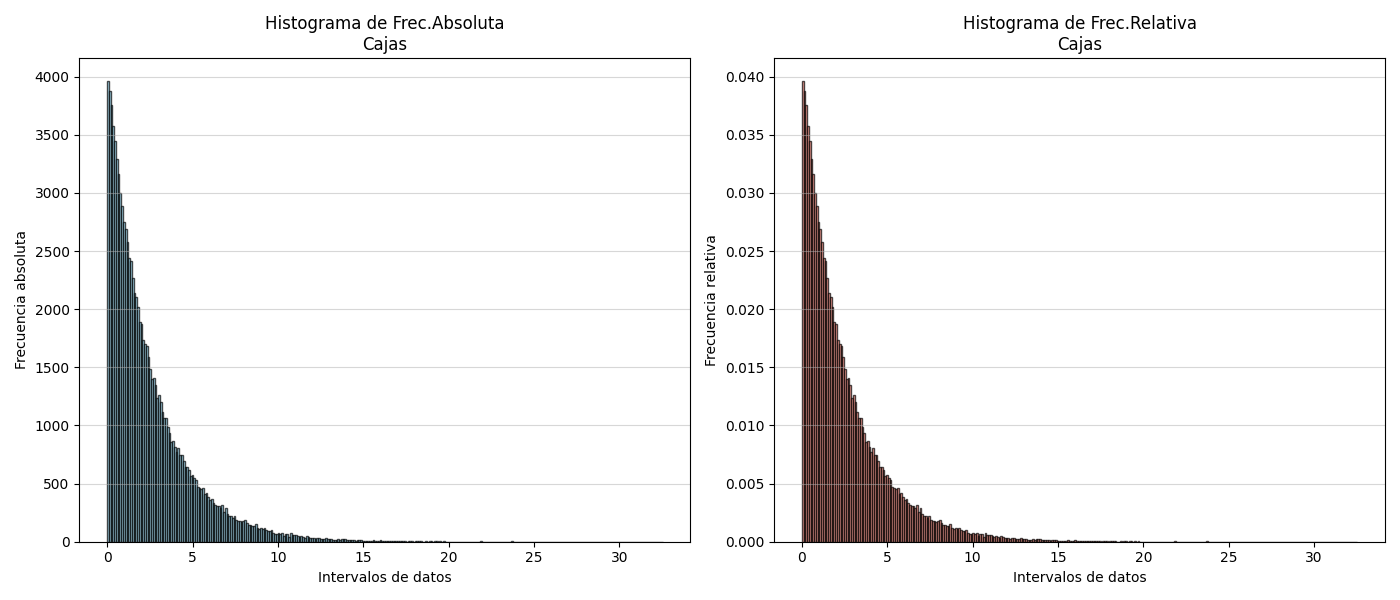
\includegraphics[width=\linewidth]{Imágenes/frec/cajaFrec.png}
        \caption{Histograma de frecuencias}
        \label{fig:frec_cajas}
    \end{subfigure}
    \quad
    \begin{subfigure}{0.40\textwidth}
        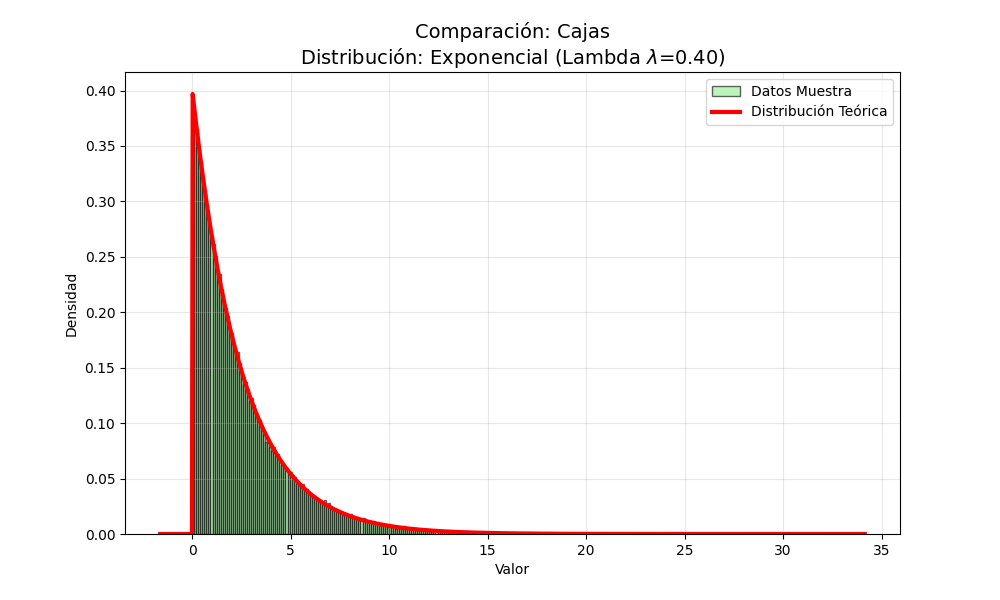
\includegraphics[width=\linewidth]{Imágenes/compara/cajaCompara.png}
        \caption{Comparación de la muestra}
        \label{fig:compara_cajas}
    \end{subfigure}
    \caption{Histogramas para el servicio de cajas.}
    \label{fig:hist_cajas}
\end{figure}

\begin{figure}[H]
    \centering
    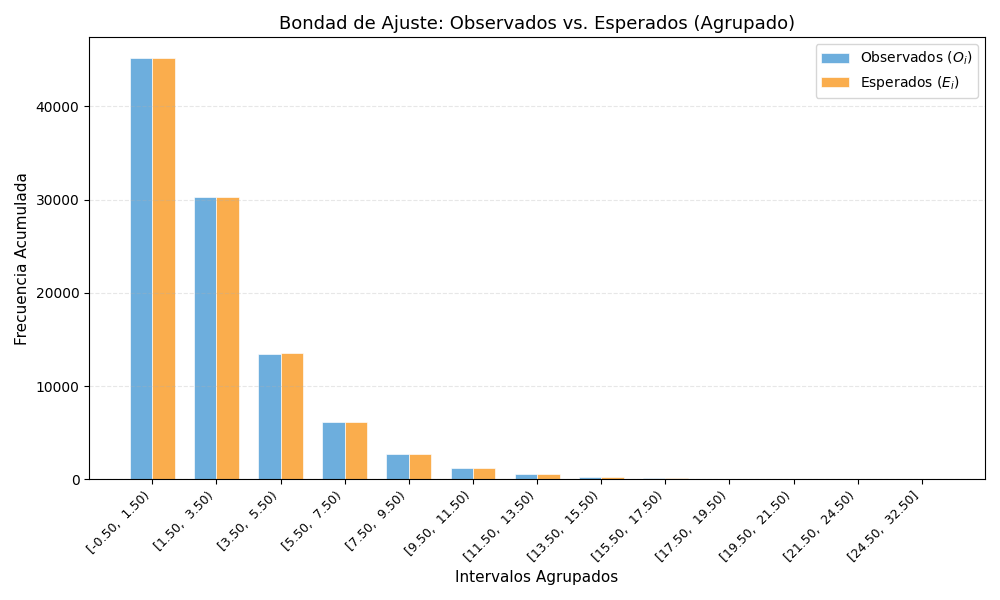
\includegraphics[width=0.5\textwidth]{Imágenes/obsEspe/cajasObsEspe.png}
    \caption{Observados vs Esperados para cajas.}
    \label{fig:obsEspe_cajas}
\end{figure}

\begin{center}
    \textbf{Datos de la muestra (Cajas):}
    \vspace{0.2cm}
    \\Media (\(\mu\)): 2.4984 \quad | \quad Lambda (\(\lambda\)): 0.40
\end{center}

\newpage
\subsubsection*{1.1.2.\hspace{0.5em} Planteamiento de hipótesis}
En base al análisis de los datos, se proponen las siguientes hipótesis:
\begin{center}
    \textbf{\(H_0\):} Esta es una distribución \textbf{Exponencial} con
    \(\lambda = 0.40\).\\[0.5em]
    \textbf{\(H_1\):} La anterior \textbf{NO} es una buena descripción
    de la distribución.
\end{center}

\vspace{0.3cm}
\noindent \textbf{Criterios de decisión:}
\begin{itemize}
    \item Para la prueba \(\chi^2\): un nivel de confianza de \(95\%\) (\(\alpha = 0.05\)).
    \item Para la prueba \textit{Kolmogorov-Smirnov}: un nivel de confianza de \(95\%\) (\(\alpha = 0.05\)).
    \item Si \(\chi^2 \leq \text{valorCritico}\) y \(d \leq \text{valorCritico}\), entonces se acepta \(H_0\).
    \item Si no se cumple lo anterior, se rechaza la hipótesis nula.
\end{itemize}
\vspace{0.3cm}

\subsubsection*{1.1.3.\hspace{0.5em} Pruebas de bondad de ajuste}
\vspace{0.2cm}
\begin{minipage}{0.40\textwidth}
    \textbf{Función de Densidad (PDF):}
    \[
        f(x) = \lambda e^{-\lambda x}, \quad x \ge 0
    \]
\end{minipage}
\begin{minipage}{0.45\textwidth}
    \textbf{Función de Distribución (CDF):}
    \[
        F(x) = 1 - e^{-\lambda x}, \quad x \ge 0
    \]
\end{minipage}
\vspace{0.3cm}

\noindent
\begin{minipage}[t]{0.48\textwidth}
    \textbf{1. Prueba de \(\chi^2\)}
    \vspace{0.3cm}
    \begin{itemize}[itemsep=0.4em]
        \item \textbf{Calculado \(\chi^2\):} 27.4483
        \item \textbf{Valor crítico:} 43.7730
    \end{itemize}

    \begin{center}
        \vspace{0.5cm}
        \(27.4483 \leq 43.7730\)
        \vspace{0.1cm}
        \\\textbf{Resultado: }
        \textcolor{green!60!black}{\textbf{Aprobado}}
    \end{center}

    \vspace{0.8cm}

    \textbf{2. Prueba de Kolmogorov--Smirnov}
    \vspace{0.3cm}
    \begin{itemize}[itemsep=0.4em]
        \item \textbf{Calculado \(D\):} 0.001403
        \item \textbf{Valor crítico:} 0.004301
    \end{itemize}
    \begin{center}
        \vspace{0.5cm}
        \(0.0014 \leq 0.0043\)
        \vspace{0.1cm}
        \\\textbf{Resultado: }
        \textcolor{green!60!black}{\textbf{Aprobado}}
    \end{center}

\end{minipage}
\hfill
\begin{minipage}[t]{0.48\textwidth}
    \vspace{0pt}
    \centering
    \begin{tikzpicture}
        \begin{axis}[
                width=\textwidth,
                height=6cm,
                title={Distribución del estadístico \(\chi^2\) (Cajas)},
                xlabel={Valor de \(\chi^2\)},
                ylabel={Densidad},
                xmin=0, xmax=60,
                ymin=0, ymax=1.1,
                grid=both,
                domain=0:60,
                samples=100,
                label style={font=\footnotesize},
                tick label style={font=\footnotesize},
                legend style={
                        nodes={scale=0.8, transform shape},
                        at={(0.98,0.98)},
                        anchor=north east
                    },]
            \addplot[blue, thick, smooth]
            {exp(-0.5*((x-25)/10)^2)};
            \addlegendentry{Distribución \(\chi^2\)}
            \addplot[red, thick]
            coordinates {(43.7729, 0) (43.7729, 1)};
            \addlegendentry{Crítico (43.77)}
            \addplot[fill=red, opacity=0.1]
            coordinates {(43.7729, 0) (60, 0) (60, 1) (43.7729, 1)};
            \addplot[
                mark=*,
                only marks,
                mark options={color=green!60!black, fill=green!60!black}
            ] coordinates {(27.4483, 0.1)};
        \end{axis}
    \end{tikzpicture}
\end{minipage}
\vspace{0.5cm}

\begin{center}
    Dado que ambas pruebas fueron aprobadas,
    \textbf{se acepta \(H_0\)}.
\end{center}


% Refrescos
\subsection{Servidor refrescos}
\subsubsection*{1.2.1.\hspace{0.5em} Análisis de frecuencias}
\begin{figure}[H]
    \centering
    \begin{subfigure}{0.55\textwidth}
        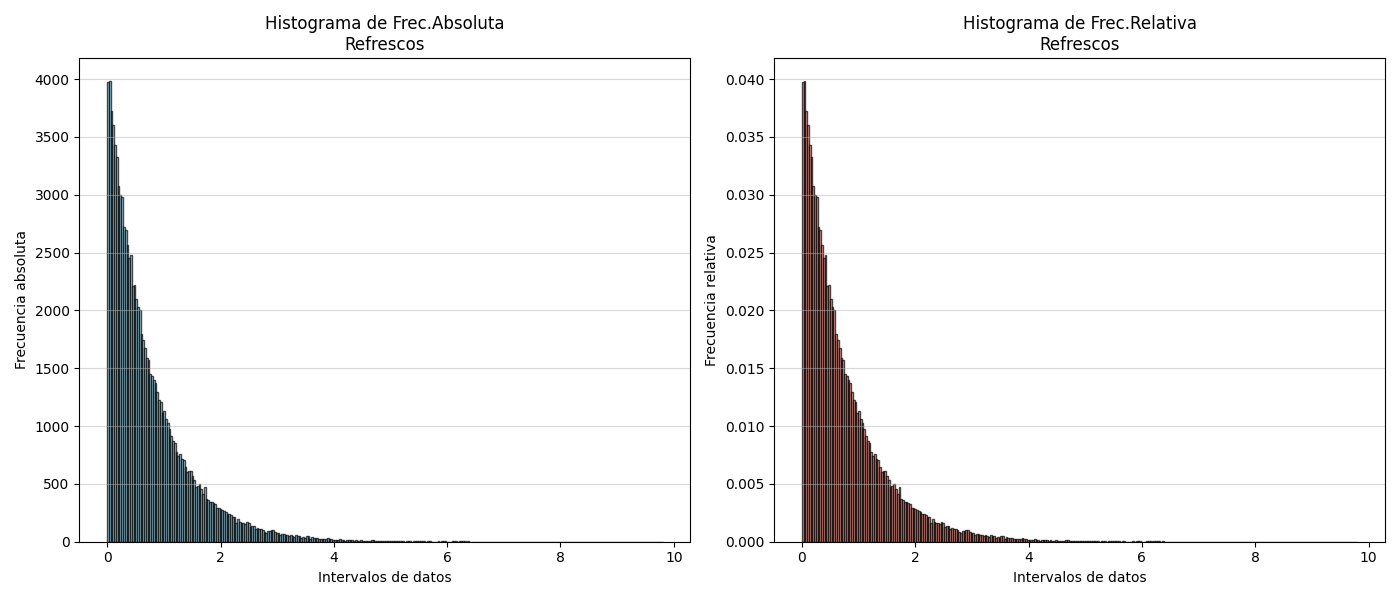
\includegraphics[width=\linewidth]{Imágenes/frec/refreFrec.png}
        \caption{Histograma de frecuencias}
        \label{fig:frec_refrescos}
    \end{subfigure}
    \quad
    \begin{subfigure}{0.40\textwidth}
        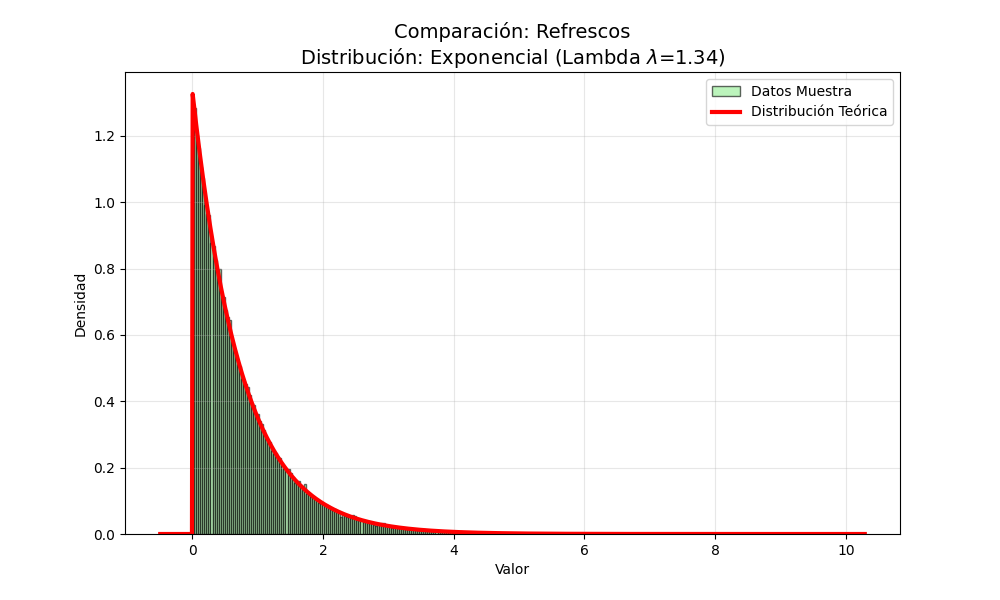
\includegraphics[width=\linewidth]{Imágenes/compara/refreCompara.png}
        \caption{Comparación de la muestra}
        \label{fig:compara_refrescos}
    \end{subfigure}
    \caption{Histogramas para el servicio de refrescos.}
    \label{fig:hist_refrescos}
\end{figure}

\begin{figure}[H]
    \centering
    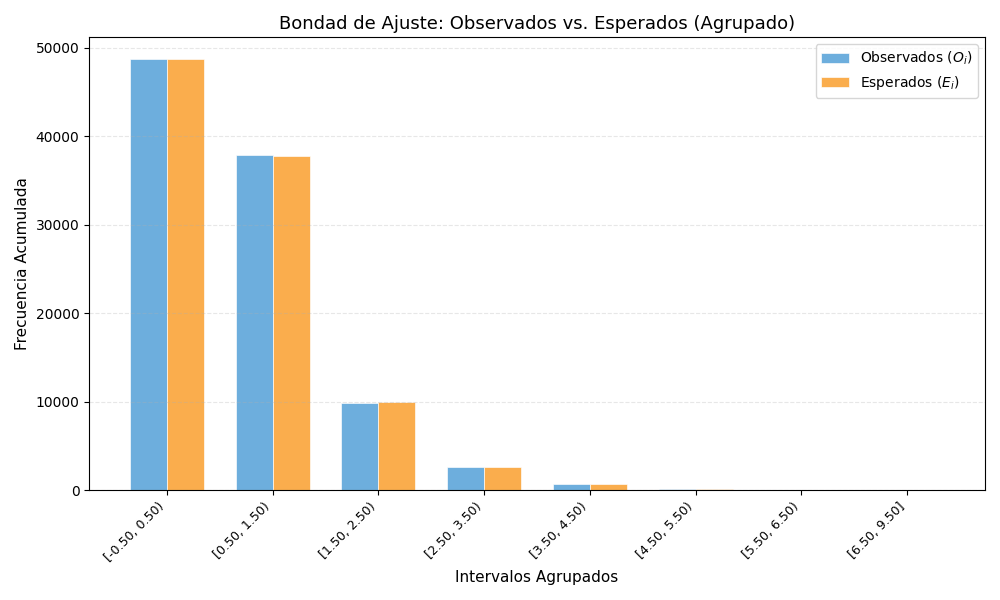
\includegraphics[width=0.5\textwidth]{Imágenes/obsEspe/refreObsEspe.png}
    \caption{Observados vs Esperados para refrescos.}
    \label{fig:obsEspe_refrescos}
\end{figure}

\begin{center}
    \textbf{Datos de la muestra (Refrescos):}
    \vspace{0.2cm}
    \\Media (\(\mu\)): 0.7477 \quad | \quad Lambda (\(\lambda\)): 1.34
\end{center}

\newpage
\subsubsection*{1.2.2.\hspace{0.5em} Planteamiento de hipótesis}
En base al análisis de los datos, se proponen las siguientes hipótesis:
\begin{center}
    \textbf{\(H_0\):} Esta es una distribución \textbf{Exponencial} con
    \(\lambda = 1.34\).\\[0.5em]
    \textbf{\(H_1\):} La anterior \textbf{NO} es una buena descripción
    de la distribución.
\end{center}

\vspace{0.3cm}
\noindent \textbf{Criterios de decisión:}
\begin{itemize}
    \item Para la prueba \(\chi^2\): un nivel de confianza de \(95\%\) (\(\alpha = 0.05\)).
    \item Para la prueba \textit{Kolmogorov-Smirnov}: un nivel de confianza de \(95\%\) (\(\alpha = 0.05\)).
    \item Si \(\chi^2 \leq \text{valorCritico}\) y \(d \leq \text{valorCritico}\), entonces se acepta \(H_0\).
    \item Si no se cumple lo anterior, se rechaza la hipótesis nula.
\end{itemize}
\vspace{0.3cm}

\subsubsection*{1.2.3.\hspace{0.5em} Pruebas de bondad de ajuste}
\vspace{0.2cm}
\begin{minipage}{0.40\textwidth}
    \textbf{Función de Densidad (PDF):}
    \[
        f(x) = \lambda e^{-\lambda x}, \quad x \ge 0
    \]
\end{minipage}
\begin{minipage}{0.45\textwidth}
    \textbf{Función de Distribución (CDF):}
    \[
        F(x) = 1 - e^{-\lambda x}, \quad x \ge 0
    \]
\end{minipage}
\vspace{0.3cm}

\noindent
\begin{minipage}[t]{0.48\textwidth}
    \textbf{1. Prueba de \(\chi^2\)}
    \vspace{0.3cm}
    \begin{itemize}[itemsep=0.4em]
        \item \textbf{Calculado \(\chi^2\):} 5.4405
        \item \textbf{Valor crítico:} 14.0671
    \end{itemize}

    \begin{center}
        \vspace{0.5cm}
        \(5.4405 \leq 14.0671\)
        \vspace{0.1cm}
        \\\textbf{Resultado: }
        \textcolor{green!60!black}{\textbf{Aprobado}}
    \end{center}

    \vspace{0.8cm}

    \textbf{2. Prueba de Kolmogorov--Smirnov}
    \vspace{0.3cm}
    \begin{itemize}[itemsep=0.4em]
        \item \textbf{Calculado \(D\):} 0.001934
        \item \textbf{Valor crítico:} 0.004301
    \end{itemize}
    \begin{center}
        \vspace{0.5cm}
        \(0.0019 \leq 0.0043\)
        \vspace{0.1cm}
        \\\textbf{Resultado: }
        \textcolor{green!60!black}{\textbf{Aprobado}}
    \end{center}

\end{minipage}
\hfill
\begin{minipage}[t]{0.48\textwidth}
    \vspace{0pt}
    \centering
    \begin{tikzpicture}
        \begin{axis}[
                width=\textwidth,
                height=6cm,
                title={Distribución del estadístico \(\chi^2\) (Refrescos)},
                xlabel={Valor de \(\chi^2\)},
                ylabel={Densidad},
                xmin=0, xmax=25,
                ymin=0, ymax=1.1,
                grid=both,
                domain=0:25,
                samples=100,
                label style={font=\footnotesize},
                tick label style={font=\footnotesize},
                legend style={
                        nodes={scale=0.8, transform shape},
                        at={(0.98,0.98)},
                        anchor=north east
                    },]
            \addplot[blue, thick, smooth]
            {exp(-0.5*((x-7)/3.5)^2)};
            \addlegendentry{Distribución \(\chi^2\)}
            \addplot[red, thick]
            coordinates {(14.0671, 0) (14.0671, 1)};
            \addlegendentry{Crítico (14.07)}
            \addplot[fill=red, opacity=0.1]
            coordinates {(14.0671, 0) (25, 0) (25, 1) (14.0671, 1)};
            \addplot[
                mark=*,
                only marks,
                mark options={color=green!60!black, fill=green!60!black}
            ] coordinates {(5.4405, 0.1)};
        \end{axis}
    \end{tikzpicture}
\end{minipage}
\vspace{0.5cm}

\begin{center}
    Dado que ambas pruebas fueron aprobadas,
    \textbf{se acepta \(H_0\)}.
\end{center}


% Llegadas
\subsection{Servidor llegadas}
\subsubsection*{1.3.1.\hspace{0.5em} Análisis de frecuencias}
\begin{figure}[H]
    \centering
    \begin{subfigure}{0.55\textwidth}
        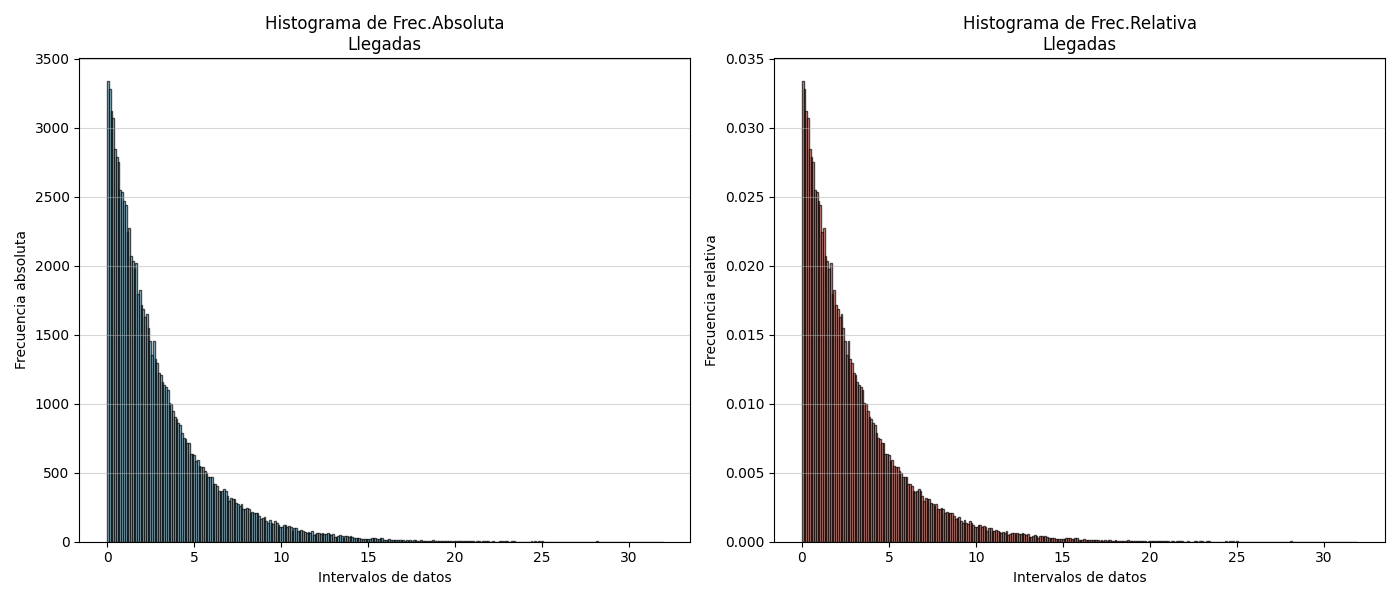
\includegraphics[width=\linewidth]{Imágenes/frec/llegadaFrec.png}
        \caption{Histograma de frecuencias}
        \label{fig:frec_llegadas}
    \end{subfigure}
    \quad
    \begin{subfigure}{0.40\textwidth}
        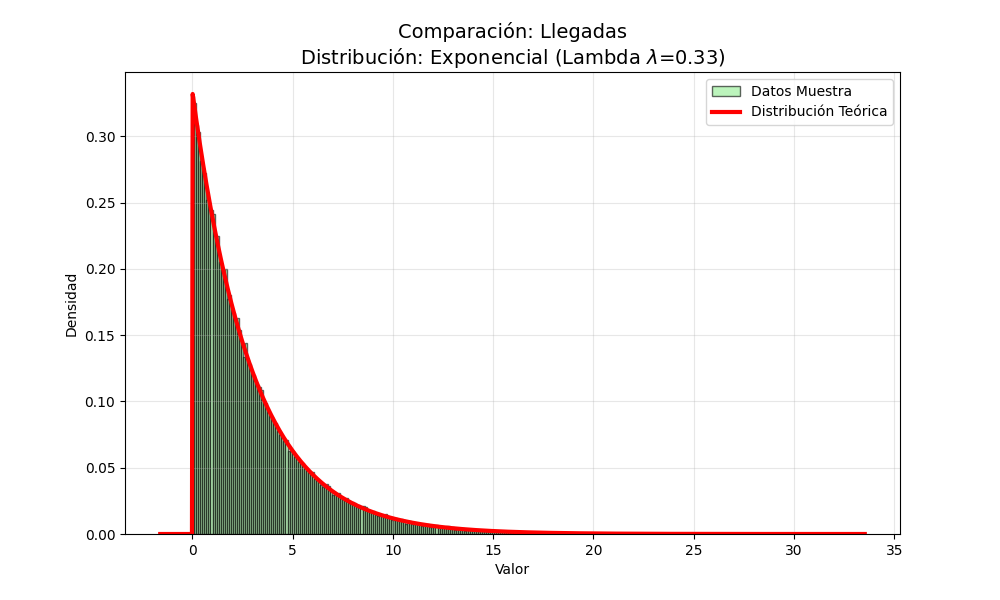
\includegraphics[width=\linewidth]{Imágenes/compara/llegadaCompara.png}
        \caption{Comparación de la muestra}
        \label{fig:compara_llegadas}
    \end{subfigure}
    \caption{Histogramas para el servicio de llegadas.}
    \label{fig:hist_llegadas}
\end{figure}

\begin{figure}[H]
    \centering
    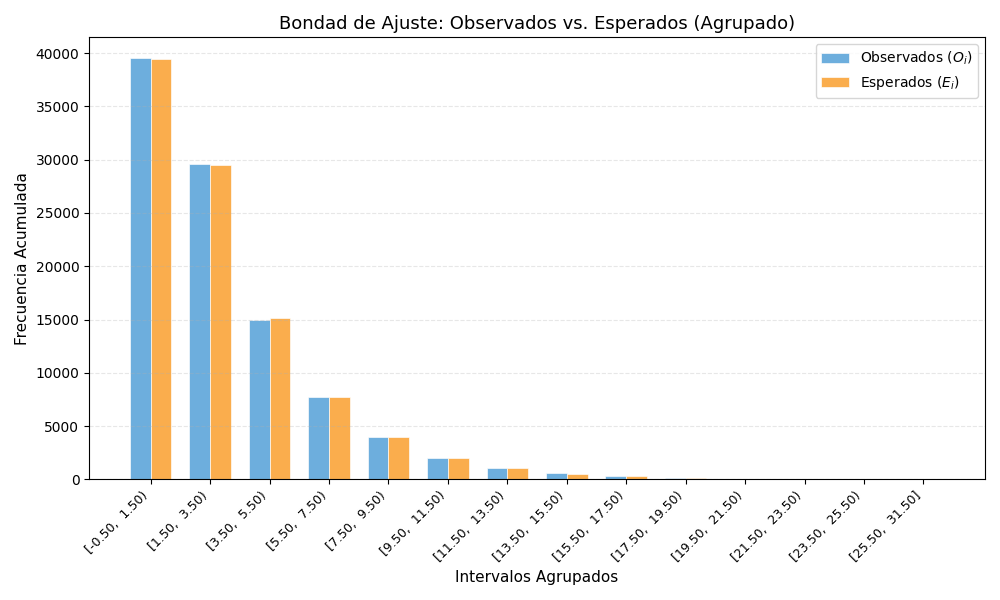
\includegraphics[width=0.5\textwidth]{Imágenes/obsEspe/llegadaObsEspe.png}
    \caption{Observados vs Esperados para llegadas.}
    \label{fig:obsEspe_llegadas}
\end{figure}

\begin{center}
    \textbf{Datos de la muestra (Llegadas):}
    \vspace{0.2cm}
    \\Media (\(\mu\)): 2.9913 \quad | \quad Lambda (\(\lambda\)): 0.33
\end{center}

\newpage
\subsubsection*{1.3.2.\hspace{0.5em} Planteamiento de hipótesis}
En base al análisis de los datos, se proponen las siguientes hipótesis:
\begin{center}
    \textbf{\(H_0\):} Esta es una distribución \textbf{Exponencial} con
    \(\lambda = 0.33\).\\[0.5em]
    \textbf{\(H_1\):} La anterior \textbf{NO} es una buena descripción
    de la distribución.
\end{center}

\vspace{0.3cm}
\noindent \textbf{Criterios de decisión:}
\begin{itemize}
    \item Para la prueba \(\chi^2\): un nivel de confianza de \(95\%\) (\(\alpha = 0.05\)).
    \item Para la prueba \textit{Kolmogorov-Smirnov}: un nivel de confianza de \(95\%\) (\(\alpha = 0.05\)).
    \item Si \(\chi^2 \leq \text{valorCritico}\) y \(d \leq \text{valorCritico}\), entonces se acepta \(H_0\).
    \item Si no se cumple lo anterior, se rechaza la hipótesis nula.
\end{itemize}
\vspace{0.3cm}

\subsubsection*{1.3.3.\hspace{0.5em} Pruebas de bondad de ajuste}
\vspace{0.2cm}
\begin{minipage}{0.40\textwidth}
    \textbf{Función de Densidad (PDF):}
    \[
        f(x) = \lambda e^{-\lambda x}, \quad x \ge 0
    \]
\end{minipage}
\begin{minipage}{0.45\textwidth}
    \textbf{Función de Distribución (CDF):}
    \[
        F(x) = 1 - e^{-\lambda x}, \quad x \ge 0
    \]
\end{minipage}
\vspace{0.3cm}

\noindent
\begin{minipage}[t]{0.48\textwidth}
    \textbf{1. Prueba de \(\chi^2\)}
    \vspace{0.3cm}
    \begin{itemize}[itemsep=0.4em]
        \item \textbf{Calculado \(\chi^2\):} 21.3846
        \item \textbf{Valor crítico:} 42.5569
    \end{itemize}

    \begin{center}
        \vspace{0.5cm}
        \(21.3846 \leq 42.5569\)
        \vspace{0.1cm}
        \\\textbf{Resultado: }
        \textcolor{green!60!black}{\textbf{Aprobado}}
    \end{center}

    \vspace{0.8cm}

    \textbf{2. Prueba de Kolmogorov--Smirnov}
    \vspace{0.3cm}
    \begin{itemize}[itemsep=0.4em]
        \item \textbf{Calculado \(D\):} 0.001950
        \item \textbf{Valor crítico:} 0.004301
    \end{itemize}
    \begin{center}
        \vspace{0.5cm}
        \(0.0019 \leq 0.0043\)
        \vspace{0.1cm}
        \\\textbf{Resultado: }
        \textcolor{green!60!black}{\textbf{Aprobado}}
    \end{center}

\end{minipage}
\hfill
\begin{minipage}[t]{0.48\textwidth}
    \vspace{0pt}
    \centering
    \begin{tikzpicture}
        \begin{axis}[
                width=\textwidth,
                height=6cm,
                title={Distribución del estadístico \(\chi^2\) (Llegadas)},
                xlabel={Valor de \(\chi^2\)},
                ylabel={Densidad},
                xmin=0, xmax=60,
                ymin=0, ymax=1.1,
                grid=both,
                domain=0:60,
                samples=100,
                label style={font=\footnotesize},
                tick label style={font=\footnotesize},
                legend style={
                        nodes={scale=0.8, transform shape},
                        at={(0.98,0.98)},
                        anchor=north east
                    },]
            \addplot[blue, thick, smooth]
            {exp(-0.5*((x-25)/12)^2)};
            \addlegendentry{Distribución \(\chi^2\)}
            \addplot[red, thick]
            coordinates {(42.5569, 0) (42.5569, 1)};
            \addlegendentry{Crítico (42.56)}
            \addplot[fill=red, opacity=0.1]
            coordinates {(42.5569, 0) (60, 0) (60, 1) (42.5569, 1)};
            \addplot[
                mark=*,
                only marks,
                mark options={color=green!60!black, fill=green!60!black}
            ] coordinates {(21.3846, 0.1)};
        \end{axis}
    \end{tikzpicture}
\end{minipage}
\vspace{0.5cm}

\begin{center}
    Dado que ambas pruebas fueron aprobadas,
    \textbf{se acepta \(H_0\)}.
\end{center}


% Postres
\subsection{Servidor postres}
\subsubsection*{1.4.1.\hspace{0.5em} Análisis de frecuencias}
\begin{figure}[H]
    \centering
    \begin{subfigure}{0.55\textwidth}
        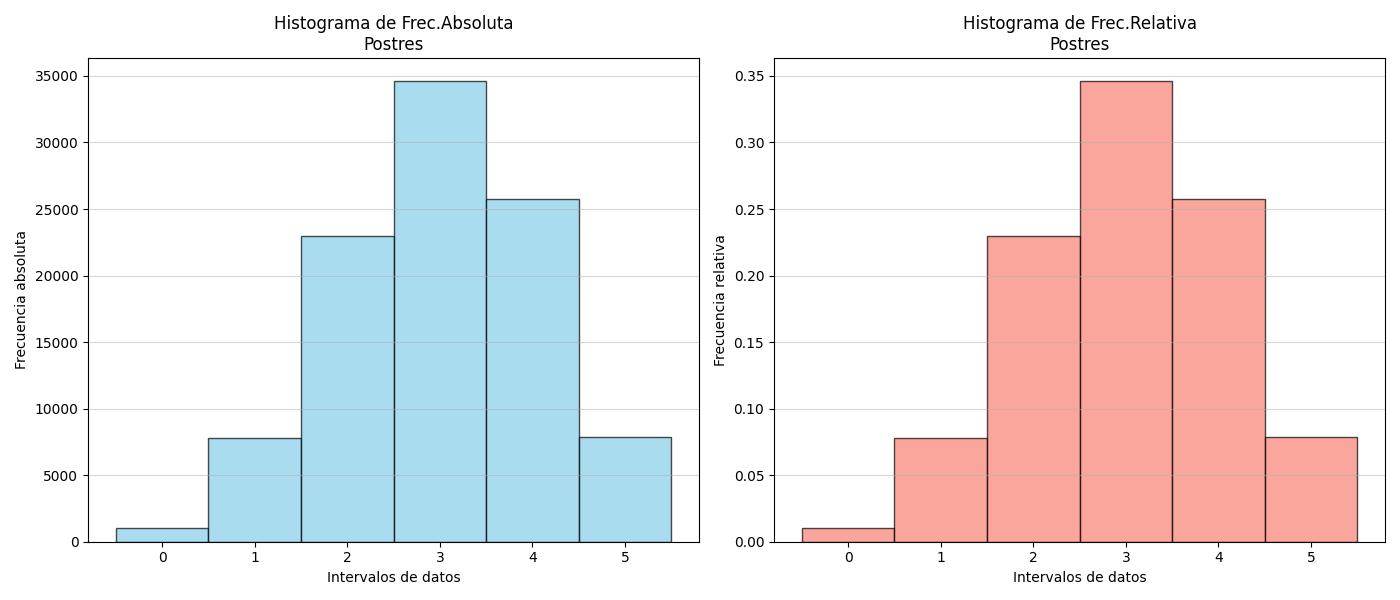
\includegraphics[width=\linewidth]{Imágenes/frec/postreFrec.png}
        \caption{Histograma de frecuencias}
        \label{fig:frec_postres}
    \end{subfigure}
    \quad
    \begin{subfigure}{0.40\textwidth}
        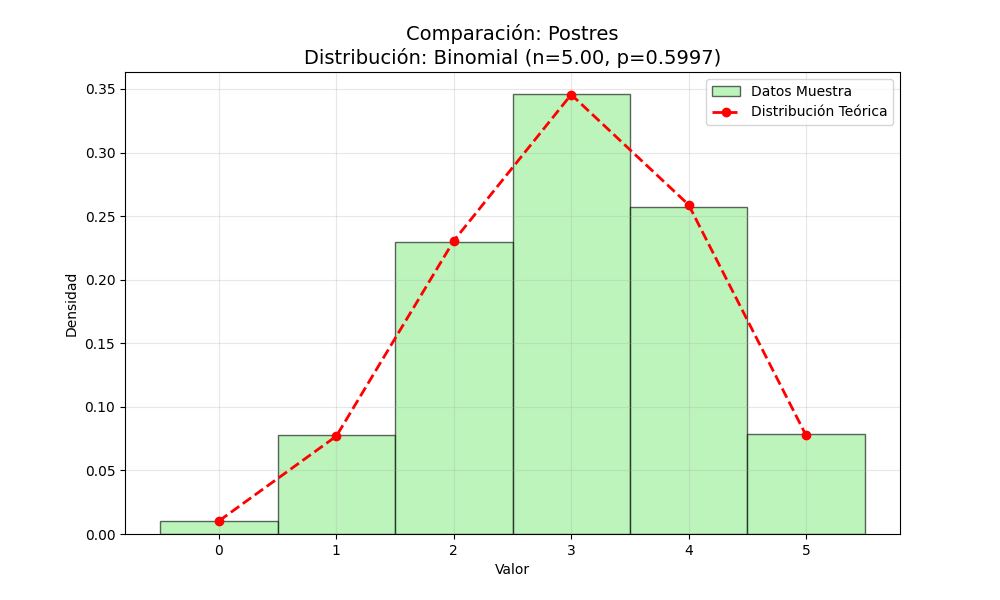
\includegraphics[width=\linewidth]{Imágenes/compara/postreCompara.png}
        \caption{Comparación de la muestra}
        \label{fig:compara_postres}
    \end{subfigure}
    \caption{Histogramas para el servicio de postres.}
    \label{fig:hist_postres}
\end{figure}

\begin{figure}[H]
    \centering
    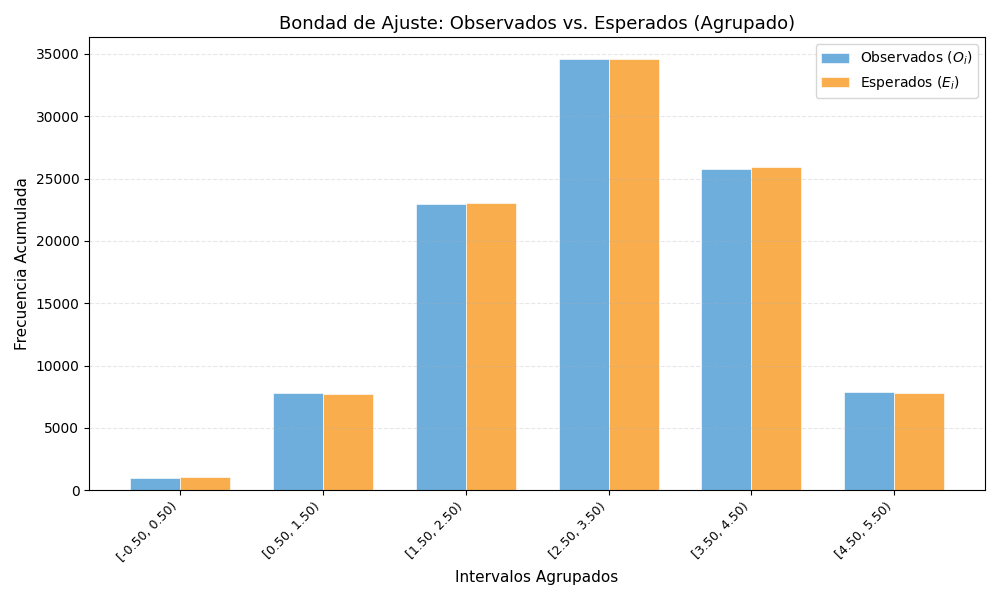
\includegraphics[width=0.5\textwidth]{Imágenes/obsEspe/postresObsEspe.png}
    \caption{Observados vs Esperados para postres.}
    \label{fig:obsEspe_postres}
\end{figure}

\begin{center}
    \textbf{Datos de la muestra (Postres):}
    \vspace{0.2cm}
    \\Parámetro (\textit{n}): 5 \quad | \quad Probabilidad (\textit{p}): 0.5997
\end{center}

\newpage
\subsubsection*{1.4.2.\hspace{0.5em} Planteamiento de hipótesis}
En base al análisis de los datos, se proponen las siguientes hipótesis:
\begin{center}
    \textbf{\(H_0\):} Esta es una distribución \textbf{Binomial} con
    \(n = 5\) y \(p = 0.5997\).\\[0.5em]
    \textbf{\(H_1\):} La anterior \textbf{NO} es una buena descripción
    de la distribución.
\end{center}

\noindent \textbf{Criterios de decisión:}
\begin{itemize}
    \item Para la prueba \(\chi^2\): un nivel de confianza de \(95\%\) (\(\alpha = 0.05\)).
    \item Para la prueba \textit{Kolmogorov-Smirnov}: un nivel de confianza de \(95\%\) (\(\alpha = 0.05\)).
    \item Si \(\chi^2 \leq \text{valorCritico}\) y \(d \leq \text{valorCritico}\), entonces se acepta \(H_0\).
    \item Si no se cumple lo anterior, se rechaza la hipótesis nula.
\end{itemize}

\subsubsection*{1.4.3.\hspace{0.5em} Pruebas de bondad de ajuste}
\vspace{0.2cm}
\begin{minipage}{0.40\textwidth}
    \textbf{Función de Masa (PMF):}
    \[
        P(X=k) = \binom{n}{k} p^k (1-p)^{n-k}
    \]
\end{minipage}
\begin{minipage}{0.45\textwidth}
    \textbf{Función de Distribución (CDF):}
    \[
        F(k) = \sum_{i=0}^{\lfloor k \rfloor} \binom{n}{i} p^i (1-p)^{n-i}
    \]
\end{minipage}

\noindent
\begin{minipage}[t]{0.48\textwidth}
    \textbf{1. Prueba de \(\chi^2\)}
    \vspace{0.3cm}
    \begin{itemize}[itemsep=0.4em]
        \item \textbf{Calculado \(\chi^2\):} 4.0657
        \item \textbf{Valor crítico:} 7.8147
    \end{itemize}

    \begin{center}
        \vspace{0.5cm}
        \(4.0657 \leq 7.8147\)
        \vspace{0.1cm}
        \\\textbf{Resultado: }
        \textcolor{green!60!black}{\textbf{Aprobado}}
    \end{center}

    \vspace{0.8cm}

    \textbf{2. Prueba de Kolmogorov--Smirnov}
    \vspace{0.3cm}
    \begin{itemize}[itemsep=0.4em]
        \item \textbf{Calculado \(D\):} 0.001106
        \item \textbf{Valor crítico:} 0.004301
    \end{itemize}
    \begin{center}
        \vspace{0.5cm}
        \(0.0011 \leq 0.0043\)
        \vspace{0.1cm}
        \\\textbf{Resultado: }
        \textcolor{green!60!black}{\textbf{Aprobado}}
    \end{center}

\end{minipage}
\hfill
\begin{minipage}[t]{0.48\textwidth}
    \vspace{0pt}
    \centering
    \begin{tikzpicture}
        \begin{axis}[
                width=\textwidth,
                height=6cm,
                title={Distribución del estadístico \(\chi^2\) (Postres)},
                xlabel={Valor de \(\chi^2\)},
                ylabel={Densidad},
                xmin=0, xmax=15,
                ymin=0, ymax=1.1,
                grid=both,
                domain=0:15,
                samples=100,
                label style={font=\footnotesize},
                tick label style={font=\footnotesize},
                legend style={
                        nodes={scale=0.8, transform shape},
                        at={(0.98,0.98)},
                        anchor=north east
                    },]
            \addplot[blue, thick, smooth]
            {exp(-0.5*((x-3.5)/2)^2)};
            \addlegendentry{Distribución \(\chi^2\)}
            \addplot[red, thick]
            coordinates {(7.8147, 0) (7.8147, 1)};
            \addlegendentry{Crítico (7.81)}
            \addplot[fill=red, opacity=0.1]
            coordinates {(7.8147, 0) (15, 0) (15, 1) (7.8147, 1)};
            \addplot[
                mark=*,
                only marks,
                mark options={color=green!60!black, fill=green!60!black}
            ] coordinates {(4.0657, 0.1)};
        \end{axis}
    \end{tikzpicture}
\end{minipage}
\vspace{0.5cm}

\begin{center}
    Dado que ambas pruebas fueron aprobadas,
    \textbf{se acepta \(H_0\)}.
\end{center}


% Ordenes
\subsection{Servidor ordenes}
\subsubsection*{1.5.1.\hspace{0.5em} Análisis de frecuencias}
\begin{figure}[H]
    \centering
    \begin{subfigure}{0.55\textwidth}
        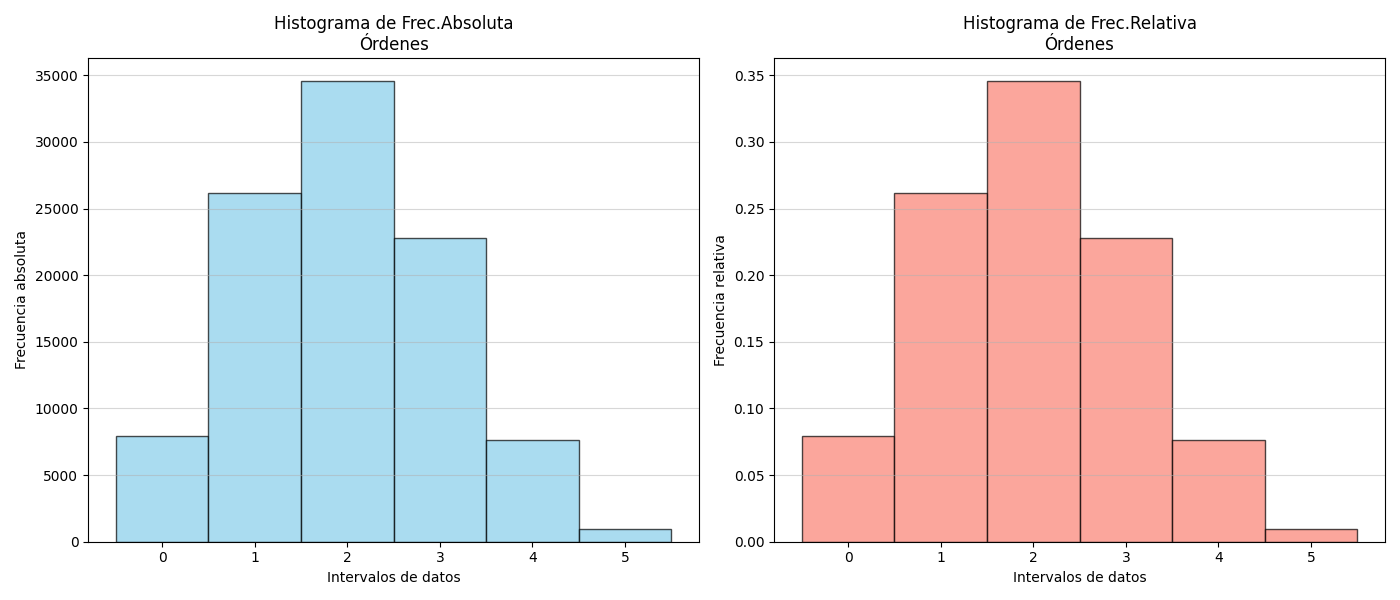
\includegraphics[width=\linewidth]{Imágenes/frec/ordenFrec.png}
        \caption{Histograma de frecuencias}
        \label{fig:frec_ordenes}
    \end{subfigure}
    \quad
    \begin{subfigure}{0.40\textwidth}
        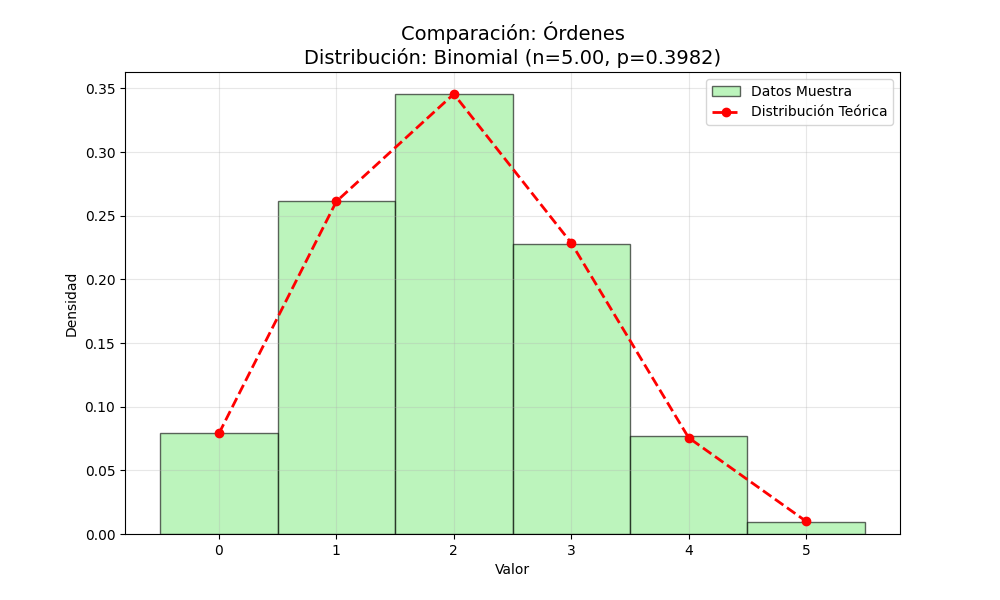
\includegraphics[width=\linewidth]{Imágenes/compara/ordenCompara.png}
        \caption{Comparación de la muestra}
        \label{fig:compara_ordenes}
    \end{subfigure}
    \caption{Histogramas para el servicio de ordenes.}
    \label{fig:hist_ordenes}
\end{figure}

\begin{figure}[H]
    \centering
    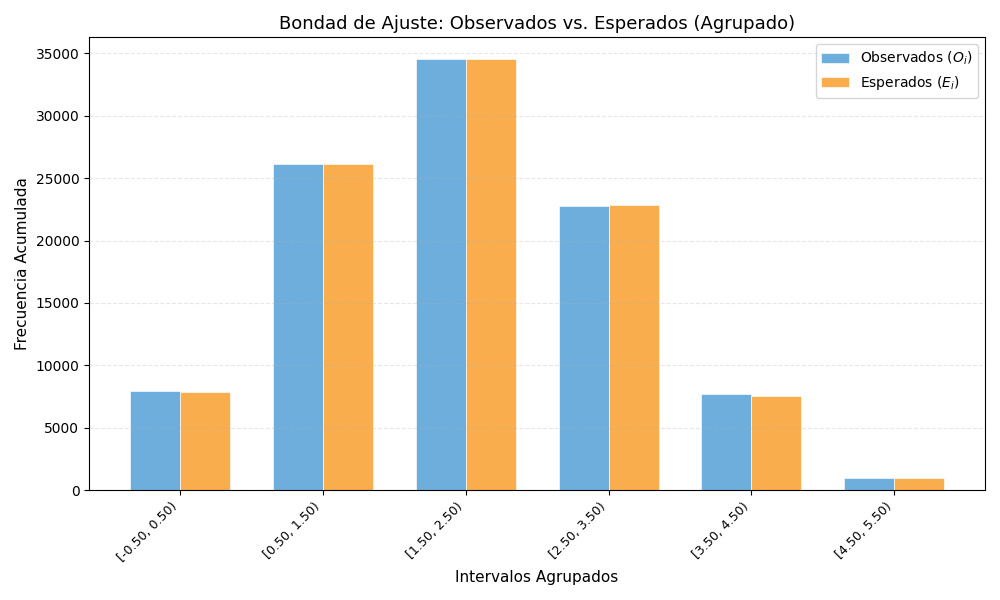
\includegraphics[width=0.5\textwidth]{Imágenes/obsEspe/ordenObsEspe.png}
    \caption{Observados vs Esperados para ordenes.}
    \label{fig:obsEspe_ordenes}
\end{figure}

\begin{center}
    \textbf{Datos de la muestra (Ordenes):}
    \vspace{0.2cm}
    \\Parámetro (\textit{n}): 5 \quad | \quad Probabilidad (\textit{p}): 0.3982
\end{center}

\newpage
\subsubsection*{1.5.2.\hspace{0.5em} Planteamiento de hipótesis}
En base al análisis de los datos, se proponen las siguientes hipótesis:
\begin{center}
    \textbf{\(H_0\):} Esta es una distribución \textbf{Binomial} con
    \(n = 5\) y \(p = 0.3982\).\\[0.5em]
    \textbf{\(H_1\):} La anterior \textbf{NO} es una buena descripción
    de la distribución.
\end{center}

\noindent \textbf{Criterios de decisión:}
\begin{itemize}
    \item Para la prueba \(\chi^2\): un nivel de confianza de \(95\%\) (\(\alpha = 0.05\)).
    \item Para la prueba \textit{Kolmogorov-Smirnov}: un nivel de confianza de \(95\%\) (\(\alpha = 0.05\)).
    \item Si \(\chi^2 \leq \text{valorCritico}\) y \(d \leq \text{valorCritico}\), entonces se acepta \(H_0\).
    \item Si no se cumple lo anterior, se rechaza la hipótesis nula.
\end{itemize}

\subsubsection*{1.5.3.\hspace{0.5em} Pruebas de bondad de ajuste}
\vspace{0.2cm}
\begin{minipage}{0.40\textwidth}
    \textbf{Función de Masa (PMF):}
    \[
        P(X=k) = \binom{n}{k} p^k (1-p)^{n-k}
    \]
\end{minipage}
\begin{minipage}{0.45\textwidth}
    \textbf{Función de Distribución (CDF):}
    \[
        F(k) = \sum_{i=0}^{\lfloor k \rfloor} \binom{n}{i} p^i (1-p)^{n-i}
    \]
\end{minipage}

\noindent
\begin{minipage}[t]{0.48\textwidth}
    \textbf{1. Prueba de \(\chi^2\)}
    \vspace{0.3cm}
    \begin{itemize}[itemsep=0.4em]
        \item \textbf{Calculado \(\chi^2\):} 2.5103
        \item \textbf{Valor crítico:} 7.8147
    \end{itemize}

    \begin{center}
        \vspace{0.5cm}
        \(2.5103 \leq 7.8147\)
        \vspace{0.1cm}
        \\\textbf{Resultado: }
        \textcolor{green!60!black}{\textbf{Aprobado}}
    \end{center}

    \vspace{0.8cm}

    \textbf{2. Prueba de Kolmogorov--Smirnov}
    \vspace{0.3cm}
    \begin{itemize}[itemsep=0.4em]
        \item \textbf{Calculado \(D\):} 0.000812
        \item \textbf{Valor crítico:} 0.004301
    \end{itemize}
    \begin{center}
        \vspace{0.5cm}
        \(0.0008 \leq 0.0043\)
        \vspace{0.1cm}
        \\\textbf{Resultado: }
        \textcolor{green!60!black}{\textbf{Aprobado}}
    \end{center}

\end{minipage}
\hfill
\begin{minipage}[t]{0.48\textwidth}
    \vspace{0pt}
    \centering
    \begin{tikzpicture}
        \begin{axis}[
                width=\textwidth,
                height=6cm,
                title={Distribución del estadístico \(\chi^2\) (Ordenes)},
                xlabel={Valor de \(\chi^2\)},
                ylabel={Densidad},
                xmin=0, xmax=15,
                ymin=0, ymax=1.1,
                grid=both,
                domain=0:15,
                samples=100,
                label style={font=\footnotesize},
                tick label style={font=\footnotesize},
                legend style={
                        nodes={scale=0.8, transform shape},
                        at={(0.98,0.98)},
                        anchor=north east
                    },]
            \addplot[blue, thick, smooth]
            {exp(-0.5*((x-3.5)/2)^2)};
            \addlegendentry{Distribución \(\chi^2\)}
            \addplot[red, thick]
            coordinates {(7.8147, 0) (7.8147, 1)};
            \addlegendentry{Crítico (7.81)}
            \addplot[fill=red, opacity=0.1]
            coordinates {(7.8147, 0) (15, 0) (15, 1) (7.8147, 1)};
            \addplot[
                mark=*,
                only marks,
                mark options={color=green!60!black, fill=green!60!black}
            ] coordinates {(2.5103, 0.1)};
        \end{axis}
    \end{tikzpicture}
\end{minipage}
\vspace{0.5cm}

\begin{center}
    Dado que ambas pruebas fueron aprobadas,
    \textbf{se acepta \(H_0\)}.
\end{center}


% Pollo
\subsection{Servidor pollo}
\subsubsection*{1.6.1.\hspace{0.5em} Análisis de frecuencias}
\begin{figure}[H]
    \centering
    \begin{subfigure}{0.55\textwidth}
        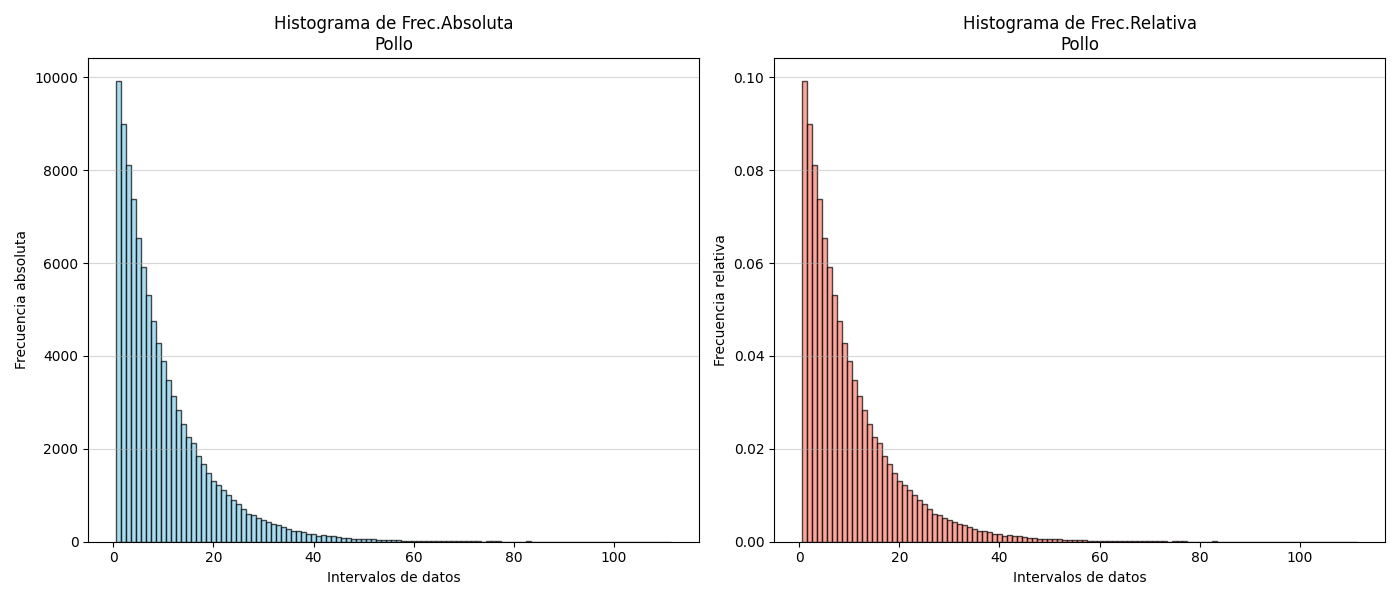
\includegraphics[width=\linewidth]{Imágenes/frec/polloFrec.png}
        \caption{Histograma de frecuencias}
        \label{fig:frec_pollo}
    \end{subfigure}
    \quad
    \begin{subfigure}{0.40\textwidth}
        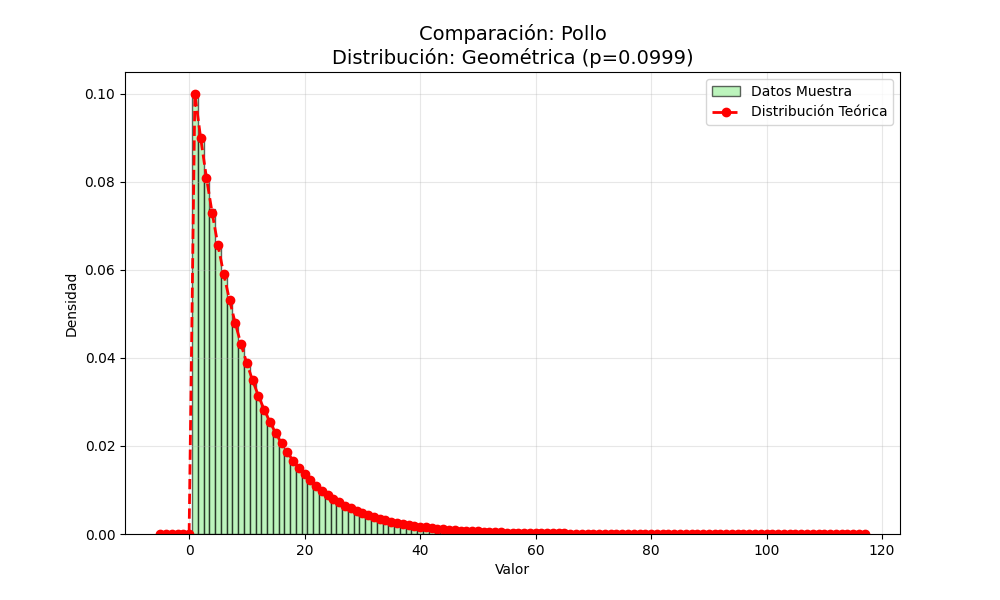
\includegraphics[width=\linewidth]{Imágenes/compara/polloCompara.png}
        \caption{Comparación de la muestra}
        \label{fig:compara_pollo}
    \end{subfigure}
    \caption{Histogramas para el servicio de pollo.}
    \label{fig:hist_pollo}
\end{figure}

\begin{figure}[H]
    \centering
    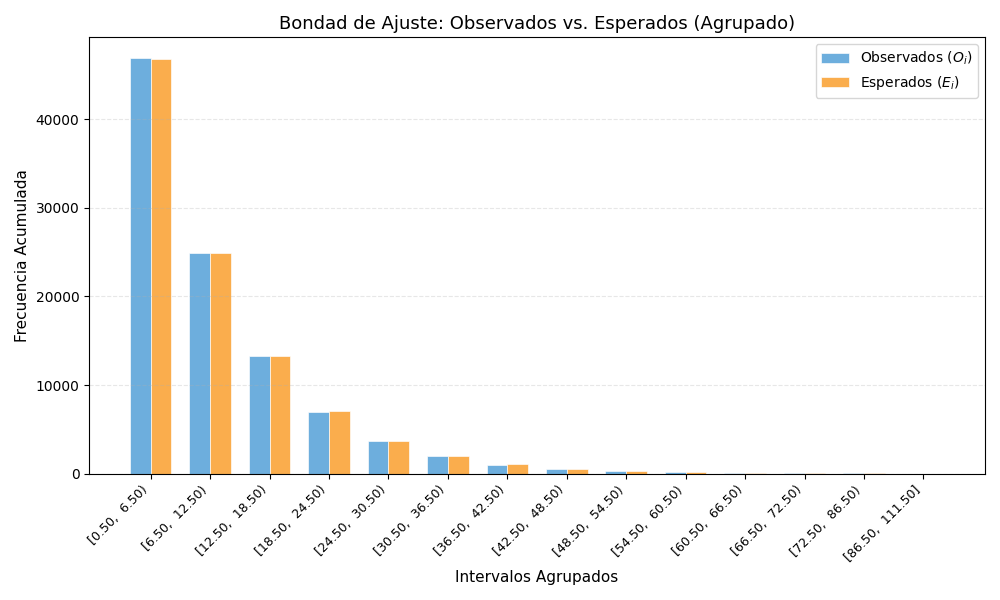
\includegraphics[width=0.5\textwidth]{Imágenes/obsEspe/polloObsEspe.png}
    \caption{Observados vs Esperados para pollo.}
    \label{fig:obsEspe_pollo}
\end{figure}

\begin{center}
    \textbf{Datos de la muestra (Pollo):}
    \vspace{0.2cm}
    \\Media (\(\mu\)): 10.0082 \quad | \quad Probabilidad (\textit{p}): 0.0999
\end{center}

\newpage
\subsubsection*{1.6.2.\hspace{0.5em} Planteamiento de hipótesis}
En base al análisis de los datos, se proponen las siguientes hipótesis:
\begin{center}
    \textbf{\(H_0\):} Esta es una distribución \textbf{Geométrica} con
    \(p = 0.0999\).\\[0.5em]
    \textbf{\(H_1\):} La anterior \textbf{NO} es una buena descripción
    de la distribución.
\end{center}

\vspace{0.3cm}
\noindent \textbf{Criterios de decisión:}
\begin{itemize}
    \item Para la prueba \(\chi^2\): un nivel de confianza de \(95\%\) (\(\alpha = 0.05\)).
    \item Para la prueba \textit{Kolmogorov-Smirnov}: un nivel de confianza de \(95\%\) (\(\alpha = 0.05\)).
    \item Si \(\chi^2 \leq \text{valorCritico}\) y \(d \leq \text{valorCritico}\), entonces se acepta \(H_0\).
    \item Si no se cumple lo anterior, se rechaza la hipótesis nula.
\end{itemize}
\vspace{0.3cm}

\subsubsection*{1.6.3.\hspace{0.5em} Pruebas de bondad de ajuste}
\vspace{0.2cm}
\begin{minipage}{0.40\textwidth}
    \textbf{Función de Masa (PMF):}
    \[
        P(X=k) = (1-p)^{k-1}p
    \]
\end{minipage}
\begin{minipage}{0.45\textwidth}
    \textbf{Función de Distribución (CDF):}
    \[
        F(k) = 1 - (1-p)^k
    \]
\end{minipage}
\vspace{0.3cm}

\noindent
\begin{minipage}[t]{0.48\textwidth}
    \textbf{1. Prueba de \(\chi^2\)}
    \vspace{0.3cm}
    \begin{itemize}[itemsep=0.4em]
        \item \textbf{Calculado \(\chi^2\):} 93.4691
        \item \textbf{Valor crítico:} 135.4802
    \end{itemize}

    \begin{center}
        \vspace{0.5cm}
        \(93.4691 \leq 135.4802\)
        \vspace{0.1cm}
        \\\textbf{Resultado: }
        \textcolor{green!60!black}{\textbf{Aprobado}}
    \end{center}

    \vspace{0.8cm}

    \textbf{2. Prueba de Kolmogorov--Smirnov}
    \vspace{0.3cm}
    \begin{itemize}[itemsep=0.4em]
        \item \textbf{Calculado \(D\):} 0.000823
        \item \textbf{Valor crítico:} 0.004301
    \end{itemize}
    \begin{center}
        \vspace{0.5cm}
        \(0.0008 \leq 0.0043\)
        \vspace{0.1cm}
        \\\textbf{Resultado: }
        \textcolor{green!60!black}{\textbf{Aprobado}}
    \end{center}

\end{minipage}
\hfill
\begin{minipage}[t]{0.48\textwidth}
    \vspace{0pt}
    \centering
    \begin{tikzpicture}
        \begin{axis}[
                width=\textwidth,
                height=6cm,
                title={Distribución del estadístico \(\chi^2\) (Pollo)},
                xlabel={Valor de \(\chi^2\)},
                ylabel={Densidad},
                xmin=50, xmax=180,
                ymin=0, ymax=1.1,
                grid=both,
                domain=50:180,
                samples=100,
                label style={font=\footnotesize},
                tick label style={font=\footnotesize},
                legend style={
                        nodes={scale=0.8, transform shape},
                        at={(0.98,0.98)},
                        anchor=north east
                    },]
            \addplot[blue, thick, smooth]
            {exp(-0.5*((x-100)/25)^2)};
            \addlegendentry{Distribución \(\chi^2\)}
            \addplot[red, thick]
            coordinates {(135.48, 0) (135.48, 1)};
            \addlegendentry{Crítico (135.48)}
            \addplot[fill=red, opacity=0.1]
            coordinates {(135.48, 0) (180, 0) (180, 1) (135.48, 1)};
            \addplot[
                mark=*,
                only marks,
                mark options={color=green!60!black, fill=green!60!black}
            ] coordinates {(93.46, 0.1)};
        \end{axis}
    \end{tikzpicture}
\end{minipage}
\vspace{0.5cm}

\begin{center}
    Dado que ambas pruebas fueron aprobadas,
    \textbf{se acepta \(H_0\)}.
\end{center}


% Freidora
\subsection{Servidor freidora}
\subsubsection*{1.7.1.\hspace{0.5em} Análisis de frecuencias}
\begin{figure}[H]
    \centering
    \begin{subfigure}{0.55\textwidth}
        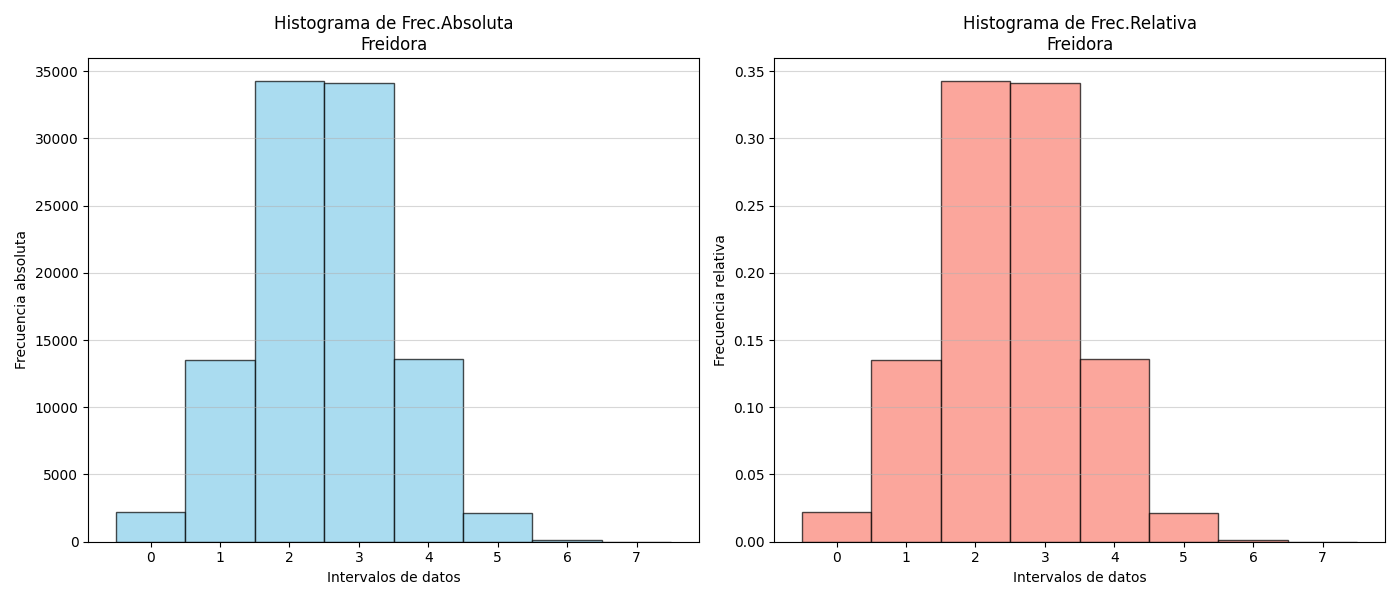
\includegraphics[width=\linewidth]{Imágenes/frec/freidoraFrec.png}
        \caption{Histograma de frecuencias}
        \label{fig:frec_freidora}
    \end{subfigure}
    \quad
    \begin{subfigure}{0.40\textwidth}
        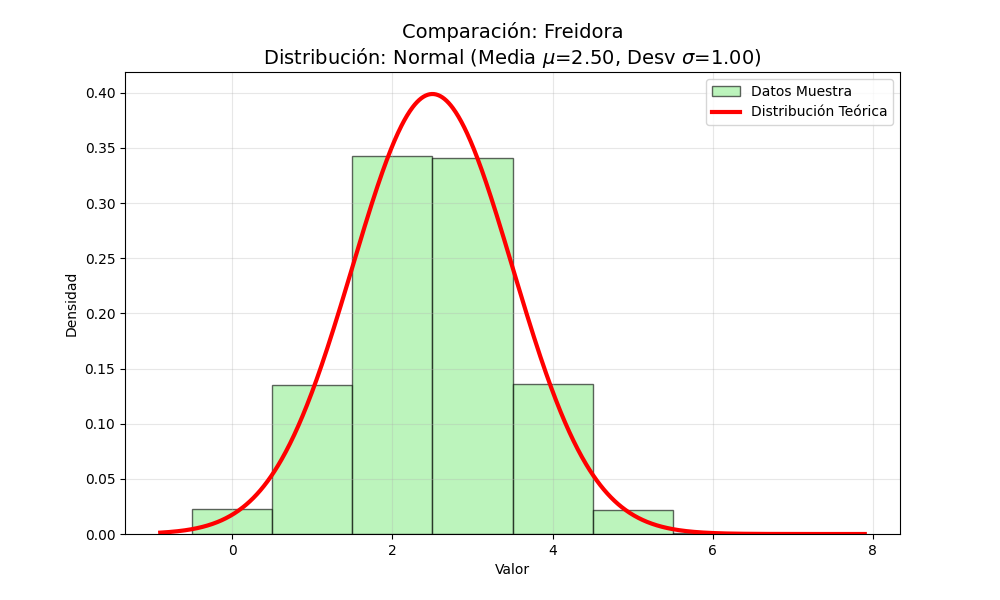
\includegraphics[width=\linewidth]{Imágenes/compara/freidoraCompara.png}
        \caption{Comparación de la muestra}
        \label{fig:compara_freidora}
    \end{subfigure}
    \caption{Histogramas para el servicio de freidora.}
    \label{fig:hist_freidora}
\end{figure}

\begin{figure}[H]
    \centering
    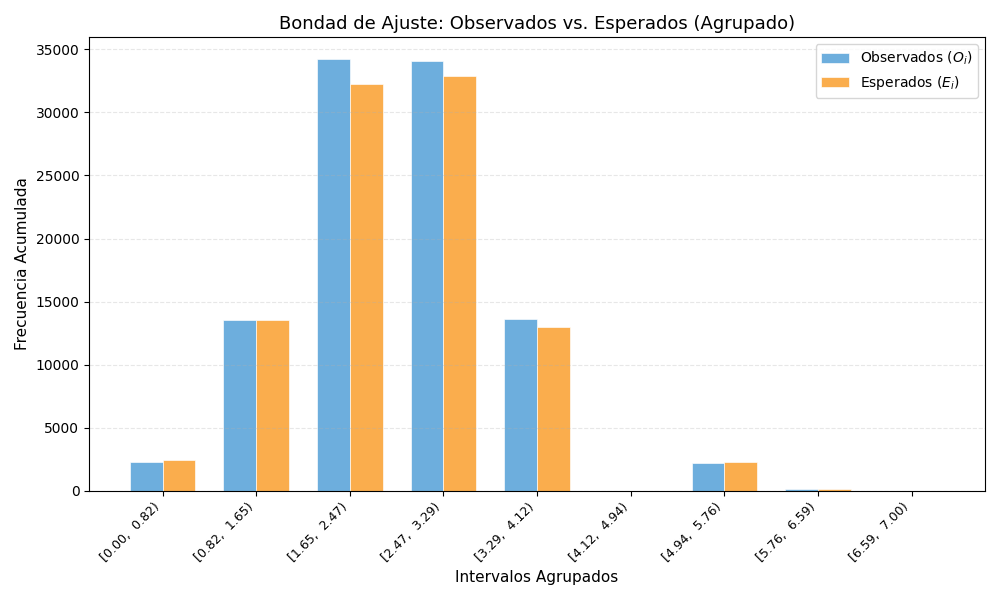
\includegraphics[width=0.5\textwidth]{Imágenes/obsEspe/freidoraObsEspe.png}
    \caption{Observados vs Esperados para freidora.}
    \label{fig:obsEspe_freidora}
\end{figure}

\begin{center}
    \textbf{Datos de la muestra (Freidora):}
    \vspace{0.2cm}
    \\Media (\(\mu\)): 2.5029 \quad | \quad Desviación (\(\sigma\)): 1.0351
\end{center}

\newpage
\subsubsection*{1.7.2.\hspace{0.5em} Planteamiento de hipótesis}
En base al análisis de los datos, se proponen las siguientes hipótesis:
\begin{center}
    \textbf{\(H_0\):} Esta es una distribución \textbf{Normal Discreta} con
    \(\mu = 2.5029\) y \(\sigma = 1.0351\).\\[0.5em]
    \textbf{\(H_1\):} La anterior \textbf{NO} es una buena descripción
    de la distribución.
\end{center}

\vspace{0.3cm}
\noindent \textbf{Criterios de decisión:}
\begin{itemize}
    \item Para la prueba \(\chi^2\): un nivel de confianza de \(95\%\) (\(\alpha = 0.05\)).
    \item Para la prueba \textit{Kolmogorov-Smirnov}: un nivel de confianza de \(95\%\) (\(\alpha = 0.05\)).
    \item Si \(\chi^2 \leq \text{valorCritico}\) y \(d \leq \text{valorCritico}\), entonces se acepta \(H_0\).
    \item Si no se cumple lo anterior, se rechaza la hipótesis nula.
\end{itemize}

\subsubsection*{1.7.3.\hspace{0.5em} Pruebas de bondad de ajuste}
\vspace{0.2cm}
\begin{minipage}{0.40\textwidth}
    \textbf{Probabilidad de Masa (PMF):}
    \[
        P(X=x) \approx \int_{x-0.5}^{x+0.5} \phi(t; \mu, \sigma) dt
    \]
\end{minipage}
\begin{minipage}{0.45\textwidth}
    \textbf{Función de Distribución (CDF):}
    \[
        F(x) \approx \Phi\left(\frac{x+0.5-\mu}{\sigma}\right)
    \]
\end{minipage}

\noindent
\begin{minipage}[t]{0.48\textwidth}
    \textbf{1. Prueba de \(\chi^2\)}
    \vspace{0.3cm}
    \begin{itemize}[itemsep=0.4em]
        \item \textbf{Calculado \(\chi^2\):} 3.8954
        \item \textbf{Valor crítico:} 11.0705
    \end{itemize}

    \begin{center}
        \vspace{0.5cm}
        \(3.8954 \leq 11.0705\)
        \vspace{0.1cm}
        \\\textbf{Resultado: }
        \textcolor{green!60!black}{\textbf{Aprobado}}
    \end{center}

    \vspace{0.8cm}

    \textbf{2. Prueba de Kolmogorov--Smirnov}
    \vspace{0.3cm}
    \begin{itemize}[itemsep=0.4em]
        \item \textbf{Calculado \(D\):} 0.001055
        \item \textbf{Valor crítico:} 0.004301
    \end{itemize}
    \begin{center}
        \vspace{0.5cm}
        \(0.0010 \leq 0.0043\)
        \vspace{0.1cm}
        \\\textbf{Resultado: }
        \textcolor{green!60!black}{\textbf{Aprobado}}
    \end{center}

\end{minipage}
\hfill
\begin{minipage}[t]{0.48\textwidth}
    \vspace{0pt}
    \centering
    \begin{tikzpicture}
        \begin{axis}[
                width=\textwidth,
                height=6cm,
                title={Distribución del estadístico \(\chi^2\) (Freidora)},
                xlabel={Valor de \(\chi^2\)},
                ylabel={Densidad},
                xmin=0, xmax=20,
                ymin=0, ymax=1.1,
                grid=both,
                domain=0:20,
                samples=100,
                label style={font=\footnotesize},
                tick label style={font=\footnotesize},
                legend style={
                        nodes={scale=0.8, transform shape},
                        at={(0.98,0.98)},
                        anchor=north east
                    },]
            \addplot[blue, thick, smooth]
            {exp(-0.5*((x-5)/3)^2)};
            \addlegendentry{Distribución \(\chi^2\)}
            \addplot[red, thick]
            coordinates {(11.0705, 0) (11.0705, 1)};
            \addlegendentry{Crítico (11.07)}
            \addplot[fill=red, opacity=0.1]
            coordinates {(11.0705, 0) (20, 0) (20, 1) (11.0705, 1)};
            \addplot[
                mark=*,
                only marks,
                mark options={color=green!60!black, fill=green!60!black}
            ] coordinates {(3.8954, 0.1)};
        \end{axis}
    \end{tikzpicture}
\end{minipage}
\vspace{0.4cm}

\begin{center}
    Dado que ambas pruebas fueron aprobadas,
    \textbf{se acepta \(H_0\)}.
\end{center}

% Gráficas (PGFPlots)
% Gráficas generadas con TikZ/PGFPlots (sin imágenes externas)
\section{Objetivo 3: Gráficas de frecuencias y covarianzas}
% Caja de estadísticas fuera de la gráfica
\newcommand{\StatsBox}[2]{%
  \begin{center}%
    \begin{tcolorbox}[width=0.95\textwidth,colback=white,colframe=black,boxrule=0.4pt,arc=1mm,left=1.2mm,right=1.2mm,top=1mm,bottom=1mm]%
      \footnotesize \textbf{#1}\\#2
    \end{tcolorbox}%
  \end{center}%
}

% --- Captions sin float (evita "Not in outer par mode" si este archivo se incluye dentro de cajas/listas) ---
% Si ya tienes \captionof (paquete caption/capt-of), la usamos. Si no, hacemos un fallback simple que:
% 1) incrementa el contador de figuras, 2) escribe en la lista de figuras, y 3) imprime el rótulo.
\makeatletter
\newcommand{\captionofmaybe}[2]{%
  \@ifundefined{captionof}{%
    \refstepcounter{#1}%
    \addcontentsline{\csname ext@#1\endcsname}{#1}{\protect\numberline{\csname the#1\endcsname}{#2}}%
    \par\smallskip\noindent\textbf{\csname fnum@#1\endcsname.}~#2\par
  }{%
    \captionof{#1}{#2}%
  }%
}
\makeatother

% Punto a
\subsection{Punto (a)}
\par\medskip
\subsubsection*{2.1.1. \hspace{0.5em} Configuración \#1: (5, 8, 9, 9, 5)}
\begin{center}
  \small Cajas = 5, Refrescos = 8, Freidora = 9, Pollo = 9, Postres = 5\\
  \vspace{0.1cm}
  \(\bar{W} = 8.4344 \quad \sigma^2 = 72.0224 \quad Precio: 1120\)
\end{center}
\begin{tikzpicture}
  \begin{groupplot}[
      group style={group size=2 by 1, horizontal sep=1.0cm},
      width=0.45\textwidth, height=0.32\textwidth,
      xlabel={Tiempo total por cliente (min)},
      xmin=0,
    ]
    \nextgroupplot[
      title={Frecuencias absolutas},
      ylabel={Conteo},
      ymin=0,
      ymax=75,
    ]
    \addplot+[ybar interval, mark=none] table[x=edge,y=count] {Datos/punto_a_hist_abs.dat};
    \addplot+[thick, mark=none] coordinates {(9.0021,0) (9.0021,75)};
    \addplot+[thick, dashed, mark=none] coordinates {(5.6771,0) (5.6771,75)};
    \addplot+[dotted, mark=none] coordinates {(3.6868,0) (3.6868,75)};
    \addplot+[dotted, mark=none] coordinates {(10.4254,0) (10.4254,75)};
    \addplot+[dash dot, mark=none] coordinates {(2.1994,0) (2.1994,75)};
    \addplot+[dash dot, mark=none] coordinates {(24.9374,0) (24.9374,75)};
    \addplot+[densely dotted, mark=none] coordinates {(0.0220,0) (0.0220,75)};
    \addplot+[densely dotted, mark=none] coordinates {(45.0302,0) (45.0302,75)};
    \nextgroupplot[
      title={Frecuencias relativas (densidad)},
      ylabel={Densidad},
      axis y line*=right,
      yticklabel pos=right,
      ymin=0,
      ymax=0.10121,
      legend to name={LegendATop1},
      legend columns=4,
      legend style={font=\scriptsize, /tikz/every even column/.append style={column sep=0.6em}},
    ]
    \addplot+[ybar interval, mark=none] table[x=edge,y=density] {Datos/punto_a_hist_rel.dat};
    \addplot+[thick, mark=none] coordinates {(9.0021,0) (9.0021,0.10121)}; \addlegendentry{Media}
    \addplot+[thick, dashed, mark=none] coordinates {(5.6771,0) (5.6771,0.10121)}; \addlegendentry{Mediana}
    \addplot+[dotted, mark=none] coordinates {(3.6868,0) (3.6868,0.10121)}; \addlegendentry{Q1}
    \addplot+[dotted, mark=none] coordinates {(10.4254,0) (10.4254,0.10121)}; \addlegendentry{Q3}
    \addplot+[dash dot, mark=none] coordinates {(2.1994,0) (2.1994,0.10121)}; \addlegendentry{P10}
    \addplot+[dash dot, mark=none] coordinates {(24.9374,0) (24.9374,0.10121)}; \addlegendentry{P90}
    \addplot+[densely dotted, mark=none] coordinates {(0.0220,0) (0.0220,0.10121)}; \addlegendentry{Mínimo}
    \addplot+[densely dotted, mark=none] coordinates {(45.0302,0) (45.0302,0.10121)}; \addlegendentry{Máximo}
  \end{groupplot}
\end{tikzpicture}
\begin{center}
  \pgfplotslegendfromname{LegendATop1}
  \StatsBox{Estadísticas de la muestra}{N = 155\\ Media = 7.8153\\ Mediana = 5.0523\\ Varianza = 70.2414\\ Moda (entera) = 3\\ Mín/Máx = 0.1429 / 70.5071\\ Q1/Q2/Q3 = 3.5901 / 5.0523 / 8.9877\\ P10/P25/P50/P75/P90 = 1.9570 / 3.5901 / 5.0523 / 8.9877 / 19.1370}
\end{center}

\begin{tikzpicture}
  \begin{axis}[
      title={Covarianzas entre estaciones},
      width=0.78\textwidth, height=0.60\textwidth,
      view={0}{90},
      colorbar,
      colormap/viridis,
      xmin=-0.5, xmax=4.5, ymin=-0.5, ymax=4.5,
      xtick={0,1,2,3,4}, ytick={0,1,2,3,4},
      xticklabels={cajas,refrescos,freidora,pollo,postres},
      yticklabels={cajas,refrescos,freidora,pollo,postres},
      x tick label style={rotate=45, anchor=east, font=\scriptsize},
      y tick label style={font=\scriptsize},
      y dir=reverse,
      axis on top,
    ]
    \addplot[
      matrix plot*,
      mesh/cols=5,
      point meta=explicit,
      nodes near coords,
      nodes near coords style={
          /pgf/number format/fixed,
          /pgf/number format/precision=2,
          font=\scriptsize,
        },
    ] table[x=x,y=y,meta=val] {Datos/punto_a_cov.dat};
  \end{axis}
\end{tikzpicture}
\captionofmaybe{figure}{Config 1: distribución de tiempos totales por cliente y covarianzas.}
\par\medskip


% Punto B
\newpage
\subsection{Punto (b)}
\par\medskip
\subsubsection*{2.2.1. \hspace{0.5em} Configuración \#1: (1, 1, 2, 3, 5)}
\begin{center}
  \small Cajas = 1, Refrescos = 1, Freidora = 2, Pollo = 3, Postres = 5 \\
  \vspace{0.1cm}
  \(\bar{W} = 22.2069 \quad \sigma^2 = 253.9162 \quad Precio: 1950\)
  \vspace{0.2cm}
\end{center}
\begin{tikzpicture}
  \begin{groupplot}[
      group style={group size=2 by 1, horizontal sep=1.0cm},
      width=0.45\textwidth, height=0.32\textwidth,
      xlabel={Tiempo total por cliente (min)},
      xmin=0,
    ]
    \nextgroupplot[
      title={Frecuencias absolutas},
      ylabel={Conteo},
      ymin=0,
      ymax=54,
    ]
    \addplot+[ybar interval, mark=none] table[x=edge,y=count] {Datos/punto_b_top1_hist_abs.dat};
    \addplot+[thick, mark=none] coordinates {(21.6814,0) (21.6814,54)};
    \addplot+[thick, dashed, mark=none] coordinates {(20.6977,0) (20.6977,54)};
    \addplot+[dotted, mark=none] coordinates {(8.9138,0) (8.9138,54)};
    \addplot+[dotted, mark=none] coordinates {(31.8547,0) (31.8547,54)};
    \addplot+[dash dot, mark=none] coordinates {(5.8067,0) (5.8067,54)};
    \addplot+[dash dot, mark=none] coordinates {(37.5471,0) (37.5471,54)};
    \addplot+[densely dotted, mark=none] coordinates {(0.8098,0) (0.8098,54)};
    \addplot+[densely dotted, mark=none] coordinates {(85.4255,0) (85.4255,54)};
    \nextgroupplot[
      title={Frecuencias relativas (densidad)},
      ylabel={Densidad},
      axis y line*=right,
      yticklabel pos=right,
      ymin=0,
      ymax=0.040460,
      legend to name={LegendBTop1},
      legend columns=4,
      legend style={font=\scriptsize, /tikz/every even column/.append style={column sep=0.6em}},
    ]
    \addplot+[ybar interval, mark=none] table[x=edge,y=density] {Datos/punto_b_top1_hist_rel.dat};
    \addplot+[thick, mark=none] coordinates {(21.6814,0) (21.6814,0.040460)}; \addlegendentry{Media}
    \addplot+[thick, dashed, mark=none] coordinates {(20.6977,0) (20.6977,0.040460)}; \addlegendentry{Mediana}
    \addplot+[dotted, mark=none] coordinates {(8.9138,0) (8.9138,0.040460)}; \addlegendentry{Q1}
    \addplot+[dotted, mark=none] coordinates {(31.8547,0) (31.8547,0.040460)}; \addlegendentry{Q3}
    \addplot+[dash dot, mark=none] coordinates {(5.8067,0) (5.8067,0.040460)}; \addlegendentry{P10}
    \addplot+[dash dot, mark=none] coordinates {(37.5471,0) (37.5471,0.040460)}; \addlegendentry{P90}
    \addplot+[densely dotted, mark=none] coordinates {(0.8098,0) (0.8098,0.040460)}; \addlegendentry{Mínimo}
    \addplot+[densely dotted, mark=none] coordinates {(85.4255,0) (85.4255,0.040460)}; \addlegendentry{Máximo}
  \end{groupplot}
\end{tikzpicture}
\begin{center}
  \pgfplotslegendfromname{LegendBTop1}
\end{center}
\StatsBox{Estadísticas de la muestra}{N = 157\\ Media = 21.6814\\ Mediana = 20.6977\\ Varianza = 221.0437\\ Moda (entera) = 5\\ Mín/Máx = 0.8098 / 85.4255\\ Q1/Q2/Q3 = 8.9138 / 20.6977 / 31.8547\\ P10/P25/P50/P75/P90 = 5.8067 / 8.9138 / 20.6977 / 31.8547 / 37.5471}
\begin{tikzpicture}
  \begin{axis}[
      title={Covarianzas entre estaciones},
      width=0.78\textwidth, height=0.60\textwidth,
      view={0}{90},
      colorbar,
      colormap/viridis,
      point meta min=-1.558500,
      point meta max=5.584600,
      xmin=-0.5, xmax=4.5, ymin=-0.5, ymax=4.5,
      xtick={0,1,2,3,4}, ytick={0,1,2,3,4},
      xticklabels={cajas,refrescos,freidora,pollo,postres},
      yticklabels={cajas,refrescos,freidora,pollo,postres},
      x tick label style={rotate=45, anchor=east, font=\scriptsize},
      y tick label style={font=\scriptsize},
      y dir=reverse,
      axis on top,
    ]
    \addplot[
      matrix plot*,
      mesh/cols=5,
      point meta=explicit,
      nodes near coords,
      nodes near coords style={
          /pgf/number format/fixed,
          /pgf/number format/precision=2,
          font=\scriptsize,
        },
    ] table[x=x,y=y,meta=val] {Datos/punto_b_top1_cov.dat};
  \end{axis}
\end{tikzpicture}
\captionofmaybe{figure}{Config 1: distribución de tiempos totales por cliente y covarianzas.}
\par\medskip


\newpage
\par\medskip
\subsubsection*{2.2.2. \hspace{0.5em} Configuración \#2: (1, 1, 1, 5, 5)}
\begin{center}
  \small Cajas = 1, Refrescos = 1, Freidora = 1, Pollo = 5, Postres = 5 \\
  \vspace{0.1cm}
  \(\bar{W} = 50.3340 \quad \sigma^2 = 1548.6204 \quad Precio: 1950\)
  \vspace{0.2cm}
\end{center}
\begin{tikzpicture}
  \begin{groupplot}[
      group style={group size=2 by 1, horizontal sep=1.0cm},
      width=0.45\textwidth, height=0.32\textwidth,
      xlabel={Tiempo total por cliente (min)},
      xmin=0,
    ]
    \nextgroupplot[
      title={Frecuencias absolutas},
      ylabel={Conteo},
      ymin=0,
      ymax=37,
    ]
    \addplot+[ybar interval, mark=none] table[x=edge,y=count] {Datos/punto_b_top2_hist_abs.dat};
    \addplot+[thick, mark=none] coordinates {(40.4948,0) (40.4948,37)};
    \addplot+[thick, dashed, mark=none] coordinates {(40.2857,0) (40.2857,37)};
    \addplot+[dotted, mark=none] coordinates {(12.6634,0) (12.6634,37)};
    \addplot+[dotted, mark=none] coordinates {(57.2500,0) (57.2500,37)};
    \addplot+[dash dot, mark=none] coordinates {(6.6814,0) (6.6814,37)};
    \addplot+[dash dot, mark=none] coordinates {(76.6548,0) (76.6548,37)};
    \addplot+[densely dotted, mark=none] coordinates {(0.1396,0) (0.1396,37)};
    \addplot+[densely dotted, mark=none] coordinates {(108.1535,0) (108.1535,37)};
    \nextgroupplot[
      title={Frecuencias relativas (densidad)},
      ylabel={Densidad},
      axis y line*=right,
      yticklabel pos=right,
      ymin=0,
      ymax=0.022374,
      legend to name={LegendBTop2},
      legend columns=4,
      legend style={font=\scriptsize, /tikz/every even column/.append style={column sep=0.6em}},
    ]
    \addplot+[ybar interval, mark=none] table[x=edge,y=density] {Datos/punto_b_top2_hist_rel.dat};
    \addplot+[thick, mark=none] coordinates {(40.4948,0) (40.4948,0.022374)}; \addlegendentry{Media}
    \addplot+[thick, dashed, mark=none] coordinates {(40.2857,0) (40.2857,0.022374)}; \addlegendentry{Mediana}
    \addplot+[dotted, mark=none] coordinates {(12.6634,0) (12.6634,0.022374)}; \addlegendentry{Q1}
    \addplot+[dotted, mark=none] coordinates {(57.2500,0) (57.2500,0.022374)}; \addlegendentry{Q3}
    \addplot+[dash dot, mark=none] coordinates {(6.6814,0) (6.6814,0.022374)}; \addlegendentry{P10}
    \addplot+[dash dot, mark=none] coordinates {(76.6548,0) (76.6548,0.022374)}; \addlegendentry{P90}
    \addplot+[densely dotted, mark=none] coordinates {(0.1396,0) (0.1396,0.022374)}; \addlegendentry{Mínimo}
    \addplot+[densely dotted, mark=none] coordinates {(108.1535,0) (108.1535,0.022374)}; \addlegendentry{Máximo}
  \end{groupplot}
\end{tikzpicture}
\begin{center}
  \pgfplotslegendfromname{LegendBTop2}
\end{center}
\StatsBox{Estadísticas de la muestra}{N = 150\\ Media = 40.4948\\ Mediana = 40.2857\\ Varianza = 750.2473\\ Moda (entera) = 12\\ Mín/Máx = 0.1396 / 108.1535\\ Q1/Q2/Q3 = 12.6634 / 40.2857 / 57.2500\\ P10/P25/P50/P75/P90 = 6.6814 / 12.6634 / 40.2857 / 57.2500 / 76.6548}
\begin{tikzpicture}
  \begin{axis}[
      title={Covarianzas entre estaciones},
      width=0.78\textwidth, height=0.60\textwidth,
      view={0}{90},
      colorbar,
      colormap/viridis,
      point meta min=-7.735700,
      point meta max=13.400000,
      xmin=-0.5, xmax=4.5, ymin=-0.5, ymax=4.5,
      xtick={0,1,2,3,4}, ytick={0,1,2,3,4},
      xticklabels={cajas,refrescos,freidora,pollo,postres},
      yticklabels={cajas,refrescos,freidora,pollo,postres},
      x tick label style={rotate=45, anchor=east, font=\scriptsize},
      y tick label style={font=\scriptsize},
      y dir=reverse,
      axis on top,
    ]
    \addplot[
      matrix plot*,
      mesh/cols=5,
      point meta=explicit,
      nodes near coords,
      nodes near coords style={
          /pgf/number format/fixed,
          /pgf/number format/precision=2,
          font=\scriptsize,
        },
    ] table[x=x,y=y,meta=val] {Datos/punto_b_top2_cov.dat};
  \end{axis}
\end{tikzpicture}
\captionofmaybe{figure}{Config 2: distribución de tiempos totales por cliente y covarianzas.}
\par\medskip

\newpage
\par\medskip
\subsubsection*{2.2.3. \hspace{0.5em} Configuración \#3: (1, 1, 3, 1, 5)}
\begin{center}
  \small Cajas = 1, Refrescos = 1, Freidora = 3, Pollo = 1, Postres = 5 \\
  \vspace{0.1cm}
  \(\bar{W} = 91.4667 \quad \sigma^2 = 23638.0594 \quad Precio: 1950\)
  \vspace{0.2cm}
\end{center}
\begin{tikzpicture}
  \begin{groupplot}[
      group style={group size=2 by 1, horizontal sep=1.0cm},
      width=0.45\textwidth, height=0.32\textwidth,
      xlabel={Tiempo total por cliente (min)},
      xmin=0,
    ]
    \nextgroupplot[
      title={Frecuencias absolutas},
      ylabel={Conteo},
      ymin=0,
      ymax=167,
    ]
    \addplot+[ybar interval, mark=none] table[x=edge,y=count] {Datos/punto_b_top3_hist_abs.dat};
    \addplot+[thick, mark=none] coordinates {(41.7874,0) (41.7874,167)};
    \addplot+[thick, dashed, mark=none] coordinates {(15.7795,0) (15.7795,167)};
    \addplot+[dotted, mark=none] coordinates {(8.7617,0) (8.7617,167)};
    \addplot+[dotted, mark=none] coordinates {(25.6127,0) (25.6127,167)};
    \addplot+[dash dot, mark=none] coordinates {(5.7578,0) (5.7578,167)};
    \addplot+[dash dot, mark=none] coordinates {(156.7378,0) (156.7378,167)};
    \addplot+[densely dotted, mark=none] coordinates {(0.6921,0) (0.6921,167)};
    \addplot+[densely dotted, mark=none] coordinates {(338.4704,0) (338.4704,167)};
    \nextgroupplot[
      title={Frecuencias relativas (densidad)},
      ylabel={Densidad},
      axis y line*=right,
      yticklabel pos=right,
      ymin=0,
      ymax=0.030382,
      legend to name={LegendBTop3},
      legend columns=4,
      legend style={font=\scriptsize, /tikz/every even column/.append style={column sep=0.6em}},
    ]
    \addplot+[ybar interval, mark=none] table[x=edge,y=density] {Datos/punto_b_top3_hist_rel.dat};
    \addplot+[thick, mark=none] coordinates {(41.7874,0) (41.7874,0.030382)}; \addlegendentry{Media}
    \addplot+[thick, dashed, mark=none] coordinates {(15.7795,0) (15.7795,0.030382)}; \addlegendentry{Mediana}
    \addplot+[dotted, mark=none] coordinates {(8.7617,0) (8.7617,0.030382)}; \addlegendentry{Q1}
    \addplot+[dotted, mark=none] coordinates {(25.6127,0) (25.6127,0.030382)}; \addlegendentry{Q3}
    \addplot+[dash dot, mark=none] coordinates {(5.7578,0) (5.7578,0.030382)}; \addlegendentry{P10}
    \addplot+[dash dot, mark=none] coordinates {(156.7378,0) (156.7378,0.030382)}; \addlegendentry{P90}
    \addplot+[densely dotted, mark=none] coordinates {(0.6921,0) (0.6921,0.030382)}; \addlegendentry{Mínimo}
    \addplot+[densely dotted, mark=none] coordinates {(338.4704,0) (338.4704,0.030382)}; \addlegendentry{Máximo}
  \end{groupplot}
\end{tikzpicture}
\begin{center}
  \pgfplotslegendfromname{LegendBTop3}
\end{center}
\StatsBox{Estadísticas de la muestra}{N = 162\\ Media = 41.7874\\ Mediana = 15.7795\\ Varianza = 4687.8525\\ Moda (entera) = 7\\ Mín/Máx = 0.6921 / 338.4704\\ Q1/Q2/Q3 = 8.7617 / 15.7795 / 25.6127\\ P10/P25/P50/P75/P90 = 5.7578 / 8.7617 / 15.7795 / 25.6127 / 156.7378}
\begin{tikzpicture}
  \begin{axis}[
      title={Covarianzas entre estaciones},
      width=0.78\textwidth, height=0.60\textwidth,
      view={0}{90},
      colorbar,
      colormap/viridis,
      point meta min=-16.605600,
      point meta max=215.876100,
      xmin=-0.5, xmax=4.5, ymin=-0.5, ymax=4.5,
      xtick={0,1,2,3,4}, ytick={0,1,2,3,4},
      xticklabels={cajas,refrescos,freidora,pollo,postres},
      yticklabels={cajas,refrescos,freidora,pollo,postres},
      x tick label style={rotate=45, anchor=east, font=\scriptsize},
      y tick label style={font=\scriptsize},
      y dir=reverse,
      axis on top,
    ]
    \addplot[
      matrix plot*,
      mesh/cols=5,
      point meta=explicit,
      nodes near coords,
      nodes near coords style={
          /pgf/number format/fixed,
          /pgf/number format/precision=2,
          font=\scriptsize,
        },
    ] table[x=x,y=y,meta=val] {Datos/punto_b_top3_cov.dat};
  \end{axis}
\end{tikzpicture}
\captionofmaybe{figure}{Config 3: distribución de tiempos totales por cliente y covarianzas.}
\par\medskip


% Punto C
\newpage
\subsection{Punto (c)}
\par\medskip
\subsubsection*{2.3.1. \hspace{0.5em}Configuración \#1: (2, 1, 3, 6, 5)}
\begin{center}
  \small Cajas = 2, Refrescos = 1, Freidora = 3, Pollo = 6, Postres = 5 \\
  \vspace{0.1cm}
  \(\bar{W} = 10.3856 \quad \sigma^2 = 71.2271 \quad Precio: 2950\)
  \vspace{0.2cm}
\end{center}
\begin{tikzpicture}
  \begin{groupplot}[
      group style={group size=2 by 1, horizontal sep=1.0cm},
      width=0.45\textwidth, height=0.32\textwidth,
      xlabel={Tiempo total por cliente (min)},
      xmin=0,
    ]
    \nextgroupplot[
      title={Frecuencias absolutas},
      ylabel={Conteo},
      ymin=0,
      ymax=78,
    ]
    \addplot+[ybar interval, mark=none] table[x=edge,y=count] {Datos/punto_c_top1_hist_abs.dat};
    \addplot+[thick, mark=none] coordinates {(11.4200,0) (11.4200,78)};
    \addplot+[thick, dashed, mark=none] coordinates {(10.3229,0) (10.3229,78)};
    \addplot+[dotted, mark=none] coordinates {(5.9867,0) (5.9867,78)};
    \addplot+[dotted, mark=none] coordinates {(14.1764,0) (14.1764,78)};
    \addplot+[dash dot, mark=none] coordinates {(3.6342,0) (3.6342,78)};
    \addplot+[dash dot, mark=none] coordinates {(20.0994,0) (20.0994,78)};
    \addplot+[densely dotted, mark=none] coordinates {(0.0543,0) (0.0543,78)};
    \addplot+[densely dotted, mark=none] coordinates {(54.0845,0) (54.0845,78)};
    \nextgroupplot[
      title={Frecuencias relativas (densidad)},
      ylabel={Densidad},
      axis y line*=right,
      yticklabel pos=right,
      ymin=0,
      ymax=0.074707,
      legend to name={LegendCTop1},
      legend columns=4,
      legend style={font=\scriptsize, /tikz/every even column/.append style={column sep=0.6em}},
    ]
    \addplot+[ybar interval, mark=none] table[x=edge,y=density] {Datos/punto_c_top1_hist_rel.dat};
    \addplot+[thick, mark=none] coordinates {(11.4200,0) (11.4200,0.074707)}; \addlegendentry{Media}
    \addplot+[thick, dashed, mark=none] coordinates {(10.3229,0) (10.3229,0.074707)}; \addlegendentry{Mediana}
    \addplot+[dotted, mark=none] coordinates {(5.9867,0) (5.9867,0.074707)}; \addlegendentry{Q1}
    \addplot+[dotted, mark=none] coordinates {(14.1764,0) (14.1764,0.074707)}; \addlegendentry{Q3}
    \addplot+[dash dot, mark=none] coordinates {(3.6342,0) (3.6342,0.074707)}; \addlegendentry{P10}
    \addplot+[dash dot, mark=none] coordinates {(20.0994,0) (20.0994,0.074707)}; \addlegendentry{P90}
    \addplot+[densely dotted, mark=none] coordinates {(0.0543,0) (0.0543,0.074707)}; \addlegendentry{Mínimo}
    \addplot+[densely dotted, mark=none] coordinates {(54.0845,0) (54.0845,0.074707)}; \addlegendentry{Máximo}
  \end{groupplot}
\end{tikzpicture}
\begin{center}
  \pgfplotslegendfromname{LegendCTop1}
\end{center}
\StatsBox{Estadísticas de la muestra}{N = 192\\ Media = 11.4200\\ Mediana = 10.3229\\ Varianza = 68.8213\\ Moda (entera) = 11\\ Mín/Máx = 0.0543 / 54.0845\\ Q1/Q2/Q3 = 5.9867 / 10.3229 / 14.1764\\ P10/P25/P50/P75/P90 = 3.6342 / 5.9867 / 10.3229 / 14.1764 / 20.0994}
\begin{tikzpicture}
  \begin{axis}[
      title={Covarianzas entre estaciones},
      width=0.78\textwidth, height=0.60\textwidth,
      view={0}{90},
      colorbar,
      colormap/viridis,
      point meta min=-1.224000,
      point meta max=8.058200,
      xmin=-0.5, xmax=4.5, ymin=-0.5, ymax=4.5,
      xtick={0,1,2,3,4}, ytick={0,1,2,3,4},
      xticklabels={cajas,refrescos,freidora,pollo,postres},
      yticklabels={cajas,refrescos,freidora,pollo,postres},
      x tick label style={rotate=45, anchor=east, font=\scriptsize},
      y tick label style={font=\scriptsize},
      y dir=reverse,
      axis on top,
    ]
    \addplot[
      matrix plot*,
      mesh/cols=5,
      point meta=explicit,
      nodes near coords,
      nodes near coords style={
          /pgf/number format/fixed,
          /pgf/number format/precision=2,
          font=\scriptsize,
        },
    ] table[x=x,y=y,meta=val] {Datos/punto_c_top1_cov.dat};
  \end{axis}
\end{tikzpicture}
\captionofmaybe{figure}{Config 1: distribución de tiempos totales por cliente y covarianzas.}
\par\medskip

\newpage
\subsubsection*{2.3.2. \hspace{0.5em} Configuración \#2: (2, 1, 4, 4, 5)}
\par\medskip
\begin{center}
  \small Cajas = 2, Refrescos = 1, Freidora = 4, Pollo = 4, Postres = 5 \\
  \vspace{0.1cm}
  \(\bar{W} = 10.8531 \quad \sigma^2 = 92.5029 \quad Precio: 2950\)
  \vspace{0.2cm}
\end{center}
\begin{tikzpicture}
  \begin{groupplot}[
      group style={group size=2 by 1, horizontal sep=1.0cm},
      width=0.45\textwidth, height=0.32\textwidth,
      xlabel={Tiempo total por cliente (min)},
      xmin=0,
    ]
    \nextgroupplot[
      title={Frecuencias absolutas},
      ylabel={Conteo},
      ymin=0,
      ymax=87,
    ]
    \addplot+[ybar interval, mark=none] table[x=edge,y=count] {Datos/punto_c_top2_hist_abs.dat};
    \addplot+[thick, mark=none] coordinates {(11.9274,0) (11.9274,87)};
    \addplot+[thick, dashed, mark=none] coordinates {(7.6954,0) (7.6954,87)};
    \addplot+[dotted, mark=none] coordinates {(5.2117,0) (5.2117,87)};
    \addplot+[dotted, mark=none] coordinates {(15.4319,0) (15.4319,87)};
    \addplot+[dash dot, mark=none] coordinates {(3.1042,0) (3.1042,87)};
    \addplot+[dash dot, mark=none] coordinates {(26.7086,0) (26.7086,87)};
    \addplot+[densely dotted, mark=none] coordinates {(0.3169,0) (0.3169,87)};
    \addplot+[densely dotted, mark=none] coordinates {(70.5495,0) (70.5495,87)};
    \nextgroupplot[
      title={Frecuencias relativas (densidad)},
      ylabel={Densidad},
      axis y line*=right,
      yticklabel pos=right,
      ymin=0,
      ymax=0.081871,
      legend to name={LegendCTop2},
      legend columns=4,
      legend style={font=\scriptsize, /tikz/every even column/.append style={column sep=0.6em}},
    ]
    \addplot+[ybar interval, mark=none] table[x=edge,y=density] {Datos/punto_c_top2_hist_rel.dat};
    \addplot+[thick, mark=none] coordinates {(11.9274,0) (11.9274,0.081871)}; \addlegendentry{Media}
    \addplot+[thick, dashed, mark=none] coordinates {(7.6954,0) (7.6954,0.081871)}; \addlegendentry{Mediana}
    \addplot+[dotted, mark=none] coordinates {(5.2117,0) (5.2117,0.081871)}; \addlegendentry{Q1}
    \addplot+[dotted, mark=none] coordinates {(15.4319,0) (15.4319,0.081871)}; \addlegendentry{Q3}
    \addplot+[dash dot, mark=none] coordinates {(3.1042,0) (3.1042,0.081871)}; \addlegendentry{P10}
    \addplot+[dash dot, mark=none] coordinates {(26.7086,0) (26.7086,0.081871)}; \addlegendentry{P90}
    \addplot+[densely dotted, mark=none] coordinates {(0.3169,0) (0.3169,0.081871)}; \addlegendentry{Mínimo}
    \addplot+[densely dotted, mark=none] coordinates {(70.5495,0) (70.5495,0.081871)}; \addlegendentry{Máximo}
  \end{groupplot}
\end{tikzpicture}
\begin{center}
  \pgfplotslegendfromname{LegendCTop2}
\end{center}
\StatsBox{Estadísticas de la muestra}{N = 150\\ Media = 11.9274\\ Mediana = 7.6954\\ Varianza = 117.1630\\ Moda (entera) = 5\\ Mín/Máx = 0.3169 / 70.5495\\ Q1/Q2/Q3 = 5.2117 / 7.6954 / 15.4319\\ P10/P25/P50/P75/P90 = 3.1042 / 5.2117 / 7.6954 / 15.4319 / 26.7086}
\begin{tikzpicture}
  \begin{axis}[
      title={Covarianzas entre estaciones},
      width=0.78\textwidth, height=0.60\textwidth,
      view={0}{90},
      colorbar,
      colormap/viridis,
      point meta min=-0.702300,
      point meta max=10.024300,
      xmin=-0.5, xmax=4.5, ymin=-0.5, ymax=4.5,
      xtick={0,1,2,3,4}, ytick={0,1,2,3,4},
      xticklabels={cajas,refrescos,freidora,pollo,postres},
      yticklabels={cajas,refrescos,freidora,pollo,postres},
      x tick label style={rotate=45, anchor=east, font=\scriptsize},
      y tick label style={font=\scriptsize},
      y dir=reverse,
      axis on top,
    ]
    \addplot[
      matrix plot*,
      mesh/cols=5,
      point meta=explicit,
      nodes near coords,
      nodes near coords style={
          /pgf/number format/fixed,
          /pgf/number format/precision=2,
          font=\scriptsize,
        },
    ] table[x=x,y=y,meta=val] {Datos/punto_c_top2_cov.dat};
  \end{axis}
\end{tikzpicture}
\captionofmaybe{figure}{Config 2: distribución de tiempos totales por cliente y covarianzas.}
\par\medskip

\newpage
\subsubsection*{2.3.3. \hspace{0.5em} Configuración \#3: (2, 1, 2, 8, 5)}
\par\medskip
\begin{center}
  \small Cajas = 2, Refrescos = 1, Freidora = 2, Pollo = 8, Postres = 5 \\
  \vspace{0.1cm}
  \(\bar{W} = 11.3973 \quad \sigma^2 = 72.7329 \quad Precio: 2950\)
  \vspace{0.2cm}
\end{center}
\begin{tikzpicture}
  \begin{groupplot}[
      group style={group size=2 by 1, horizontal sep=1.0cm},
      width=0.45\textwidth, height=0.32\textwidth,
      xlabel={Tiempo total por cliente (min)},
      xmin=0,
    ]
    \nextgroupplot[
      title={Frecuencias absolutas},
      ylabel={Conteo},
      ymin=0,
      ymax=69,
    ]
    \addplot+[ybar interval, mark=none] table[x=edge,y=count] {Datos/punto_c_top3_hist_abs.dat};
    \addplot+[thick, mark=none] coordinates {(11.2350,0) (11.2350,69)};
    \addplot+[thick, dashed, mark=none] coordinates {(9.0727,0) (9.0727,69)};
    \addplot+[dotted, mark=none] coordinates {(4.4665,0) (4.4665,69)};
    \addplot+[dotted, mark=none] coordinates {(14.8508,0) (14.8508,69)};
    \addplot+[dash dot, mark=none] coordinates {(2.3123,0) (2.3123,69)};
    \addplot+[dash dot, mark=none] coordinates {(20.3516,0) (20.3516,69)};
    \addplot+[densely dotted, mark=none] coordinates {(0.6031,0) (0.6031,69)};
    \addplot+[densely dotted, mark=none] coordinates {(67.6802,0) (67.6802,69)};
    \nextgroupplot[
      title={Frecuencias relativas (densidad)},
      ylabel={Densidad},
      axis y line*=right,
      yticklabel pos=right,
      ymin=0,
      ymax=0.073210,
      legend to name={LegendCTop3},
      legend columns=4,
      legend style={font=\scriptsize, /tikz/every even column/.append style={column sep=0.6em}},
    ]
    \addplot+[ybar interval, mark=none] table[x=edge,y=density] {Datos/punto_c_top3_hist_rel.dat};
    \addplot+[thick, mark=none] coordinates {(11.2350,0) (11.2350,0.073210)}; \addlegendentry{Media}
    \addplot+[thick, dashed, mark=none] coordinates {(9.0727,0) (9.0727,0.073210)}; \addlegendentry{Mediana}
    \addplot+[dotted, mark=none] coordinates {(4.4665,0) (4.4665,0.073210)}; \addlegendentry{Q1}
    \addplot+[dotted, mark=none] coordinates {(14.8508,0) (14.8508,0.073210)}; \addlegendentry{Q3}
    \addplot+[dash dot, mark=none] coordinates {(2.3123,0) (2.3123,0.073210)}; \addlegendentry{P10}
    \addplot+[dash dot, mark=none] coordinates {(20.3516,0) (20.3516,0.073210)}; \addlegendentry{P90}
    \addplot+[densely dotted, mark=none] coordinates {(0.6031,0) (0.6031,0.073210)}; \addlegendentry{Mínimo}
    \addplot+[densely dotted, mark=none] coordinates {(67.6802,0) (67.6802,0.073210)}; \addlegendentry{Máximo}
  \end{groupplot}
\end{tikzpicture}
\begin{center}
  \pgfplotslegendfromname{LegendCTop3}
\end{center}
\StatsBox{Estadísticas de la muestra}{N = 140\\ Media = 11.2350\\ Mediana = 9.0727\\ Varianza = 93.4119\\ Moda (entera) = 4\\ Mín/Máx = 0.6031 / 67.6802\\ Q1/Q2/Q3 = 4.4665 / 9.0727 / 14.8508\\ P10/P25/P50/P75/P90 = 2.3123 / 4.4665 / 9.0727 / 14.8508 / 20.3516}
\begin{tikzpicture}
  \begin{axis}[
      title={Covarianzas entre estaciones},
      width=0.78\textwidth, height=0.60\textwidth,
      view={0}{90},
      colorbar,
      colormap/viridis,
      point meta min=-3.405100,
      point meta max=23.232600,
      xmin=-0.5, xmax=4.5, ymin=-0.5, ymax=4.5,
      xtick={0,1,2,3,4}, ytick={0,1,2,3,4},
      xticklabels={cajas,refrescos,freidora,pollo,postres},
      yticklabels={cajas,refrescos,freidora,pollo,postres},
      x tick label style={rotate=45, anchor=east, font=\scriptsize},
      y tick label style={font=\scriptsize},
      y dir=reverse,
      axis on top,
    ]
    \addplot[
      matrix plot*,
      mesh/cols=5,
      point meta=explicit,
      nodes near coords,
      nodes near coords style={
          /pgf/number format/fixed,
          /pgf/number format/precision=2,
          font=\scriptsize,
        },
    ] table[x=x,y=y,meta=val] {Datos/punto_c_top3_cov.dat};
  \end{axis}
\end{tikzpicture}
\captionofmaybe{figure}{Config 3: distribución de tiempos totales por cliente y covarianzas.}
\par\medskip


% Punto D
\newpage
\subsection{Punto (d)}
\par\medskip
\subsubsection*{2.4.1. \hspace{0.5em} Configuración \#1: Servidores Ilimitados}
\begin{center}
  \small \(\bar{W} = 7.9343 \quad \sigma^2 = 70.1678\)
  \vspace{0.2cm}
\end{center}
\begin{tikzpicture}
  \begin{groupplot}[
      group style={group size=2 by 1, horizontal sep=1.0cm},
      width=0.45\textwidth, height=0.32\textwidth,
      xlabel={Tiempo total por cliente (min)},
      xmin=0,
    ]
    \nextgroupplot[
      title={Frecuencias absolutas},
      ylabel={Conteo},
      ymin=0,
      ymax=97,
    ]
    \addplot+[ybar interval, mark=none] table[x=edge,y=count] {Datos/punto_d_top1_hist_abs.dat};
    \addplot+[thick, mark=none] coordinates {(8.8788,0) (8.8788,97)};
    \addplot+[thick, dashed, mark=none] coordinates {(5.3395,0) (5.3395,97)};
    \addplot+[dotted, mark=none] coordinates {(3.5790,0) (3.5790,97)};
    \addplot+[dotted, mark=none] coordinates {(9.6081,0) (9.6081,97)};
    \addplot+[dash dot, mark=none] coordinates {(2.0582,0) (2.0582,97)};
    \addplot+[dash dot, mark=none] coordinates {(22.5714,0) (22.5714,97)};
    \addplot+[densely dotted, mark=none] coordinates {(0.0358,0) (0.0358,97)};
    \addplot+[densely dotted, mark=none] coordinates {(51.5574,0) (51.5574,97)};
    \nextgroupplot[
      title={Frecuencias relativas (densidad)},
      ylabel={Densidad},
      axis y line*=right,
      yticklabel pos=right,
      ymin=0,
      ymax=0.118237,
      legend to name={LegendDTop1},
      legend columns=4,
      legend style={font=\scriptsize, /tikz/every even column/.append style={column sep=0.6em}},
    ]
    \addplot+[ybar interval, mark=none] table[x=edge,y=density] {Datos/punto_d_top1_hist_rel.dat};
    \addplot+[thick, mark=none] coordinates {(8.8788,0) (8.8788,0.118237)}; \addlegendentry{Media}
    \addplot+[thick, dashed, mark=none] coordinates {(5.3395,0) (5.3395,0.118237)}; \addlegendentry{Mediana}
    \addplot+[dotted, mark=none] coordinates {(3.5790,0) (3.5790,0.118237)}; \addlegendentry{Q1}
    \addplot+[dotted, mark=none] coordinates {(9.6081,0) (9.6081,0.118237)}; \addlegendentry{Q3}
    \addplot+[dash dot, mark=none] coordinates {(2.0582,0) (2.0582,0.118237)}; \addlegendentry{P10}
    \addplot+[dash dot, mark=none] coordinates {(22.5714,0) (22.5714,0.118237)}; \addlegendentry{P90}
    \addplot+[densely dotted, mark=none] coordinates {(0.0358,0) (0.0358,0.118237)}; \addlegendentry{Mínimo}
    \addplot+[densely dotted, mark=none] coordinates {(51.5574,0) (51.5574,0.118237)}; \addlegendentry{Máximo}
  \end{groupplot}
\end{tikzpicture}
\begin{center}
  \pgfplotslegendfromname{LegendDTop1}
\end{center}
\StatsBox{Estadísticas de la muestra}{N = 158\\ Media = 8.8788\\ Mediana = 5.3395\\ Varianza = 85.4294\\ Moda (entera) = 4\\ Mín/Máx = 0.0358 / 51.5574\\ Q1/Q2/Q3 = 3.5790 / 5.3395 / 9.6081\\ P10/P25/P50/P75/P90 = 2.0582 / 3.5790 / 5.3395 / 9.6081 / 22.5714}


\par\medskip
\begin{tikzpicture}
  \begin{axis}[
      title={Covarianzas entre estaciones},
      width=0.78\textwidth, height=0.60\textwidth,
      view={0}{90},
      colorbar,
      colormap/viridis,
      point meta min=-5.174700,
      point meta max=3.603300,
      xmin=-0.5, xmax=4.5, ymin=-0.5, ymax=4.5,
      xtick={0,1,2,3,4}, ytick={0,1,2,3,4},
      xticklabels={cajas,refrescos,freidora,pollo,postres},
      yticklabels={cajas,refrescos,freidora,pollo,postres},
      x tick label style={rotate=45, anchor=east, font=\scriptsize},
      y tick label style={font=\scriptsize},
      y dir=reverse,
      axis on top,
    ]
    \addplot[
      matrix plot*,
      mesh/cols=5,
      point meta=explicit,
      nodes near coords,
      nodes near coords style={
          /pgf/number format/fixed,
          /pgf/number format/precision=2,
          font=\scriptsize,
        },
    ] table[x=x,y=y,meta=val] {Datos/punto_d_top1_cov.dat};
  \end{axis}
\end{tikzpicture}
\captionofmaybe{figure}{Config 1: distribución de tiempos totales por cliente y covarianzas.}
\par\medskip

% Punto E
\newpage
\subsection{Punto (e)}
\par\medskip
\subsubsection*{2.5.1. \hspace{0.5em} Configuración \#1: Servidores Ilimitados}
\begin{center}
  \small \(\bar{W} = 10.6112 \quad \sigma^2 = 100.6112\)
  \vspace{0.2cm}
\end{center}
\begin{tikzpicture}
  \begin{groupplot}[
      group style={group size=2 by 1, horizontal sep=1.0cm},
      width=0.45\textwidth, height=0.32\textwidth,
      xlabel={Tiempo total por cliente (min)},
      xmin=0,
    ]
    \nextgroupplot[
      title={Frecuencias absolutas},
      ylabel={Conteo},
      ymin=0,
      ymax=77,
    ]
    \addplot+[ybar interval, mark=none] table[x=edge,y=count] {Datos/punto_e_top1_hist_abs.dat};
    \addplot+[thick, mark=none] coordinates {(9.7135,0) (9.7135,77)};
    \addplot+[thick, dashed, mark=none] coordinates {(6.3785,0) (6.3785,77)};
    \addplot+[dotted, mark=none] coordinates {(3.7265,0) (3.7265,77)};
    \addplot+[dotted, mark=none] coordinates {(12.2675,0) (12.2675,77)};
    \addplot+[dash dot, mark=none] coordinates {(2.2182,0) (2.2182,77)};
    \addplot+[dash dot, mark=none] coordinates {(21.8765,0) (21.8765,77)};
    \addplot+[densely dotted, mark=none] coordinates {(0.2752,0) (0.2752,77)};
    \addplot+[densely dotted, mark=none] coordinates {(48.3704,0) (48.3704,77)};
    \nextgroupplot[
      title={Frecuencias relativas (densidad)},
      ylabel={Densidad},
      axis y line*=right,
      yticklabel pos=right,
      ymin=0,
      ymax=0.096085,
      legend to name={LegendETop1},
      legend columns=4,
      legend style={font=\scriptsize, /tikz/every even column/.append style={column sep=0.6em}},
    ]
    \addplot+[ybar interval, mark=none] table[x=edge,y=density] {Datos/punto_e_top1_hist_rel.dat};
    \addplot+[thick, mark=none] coordinates {(9.7135,0) (9.7135,0.096085)}; \addlegendentry{Media}
    \addplot+[thick, dashed, mark=none] coordinates {(6.3785,0) (6.3785,0.096085)}; \addlegendentry{Mediana}
    \addplot+[dotted, mark=none] coordinates {(3.7265,0) (3.7265,0.096085)}; \addlegendentry{Q1}
    \addplot+[dotted, mark=none] coordinates {(12.2675,0) (12.2675,0.096085)}; \addlegendentry{Q3}
    \addplot+[dash dot, mark=none] coordinates {(2.2182,0) (2.2182,0.096085)}; \addlegendentry{P10}
    \addplot+[dash dot, mark=none] coordinates {(21.8765,0) (21.8765,0.096085)}; \addlegendentry{P90}
    \addplot+[densely dotted, mark=none] coordinates {(0.2752,0) (0.2752,0.096085)}; \addlegendentry{Mínimo}
    \addplot+[densely dotted, mark=none] coordinates {(48.3704,0) (48.3704,0.096085)}; \addlegendentry{Máximo}
  \end{groupplot}
\end{tikzpicture}
\begin{center}
  \pgfplotslegendfromname{LegendETop1}
\end{center}
\StatsBox{Estadísticas de la muestra}{N = 165\\ Media = 9.7135\\ Mediana = 6.3785\\ Varianza = 75.2220\\ Moda (entera) = 3\\ Mín/Máx = 0.2752 / 48.3704\\ Q1/Q2/Q3 = 3.7265 / 6.3785 / 12.2675\\ P10/P25/P50/P75/P90 = 2.2182 / 3.7265 / 6.3785 / 12.2675 / 21.8765}
\begin{tikzpicture}
  \begin{axis}[
      title={Covarianzas entre estaciones},
      width=0.78\textwidth, height=0.60\textwidth,
      view={0}{90},
      colorbar,
      colormap/viridis,
      point meta min=-0.070500,
      point meta max=2.541300,
      xmin=-0.5, xmax=4.5, ymin=-0.5, ymax=4.5,
      xtick={0,1,2,3,4}, ytick={0,1,2,3,4},
      xticklabels={cajas,refrescos,freidora,pollo,postres},
      yticklabels={cajas,refrescos,freidora,pollo,postres},
      x tick label style={rotate=45, anchor=east, font=\scriptsize},
      y tick label style={font=\scriptsize},
      y dir=reverse,
      axis on top,
    ]
    \addplot[
      matrix plot*,
      mesh/cols=5,
      point meta=explicit,
      nodes near coords,
      nodes near coords style={
          /pgf/number format/fixed,
          /pgf/number format/precision=2,
          font=\scriptsize,
        },
    ] table[x=x,y=y,meta=val] {Datos/punto_e_top1_cov.dat};
  \end{axis}
\end{tikzpicture}
\captionofmaybe{figure}{Config 1: distribución de tiempos totales por cliente y covarianzas.}
\par\medskip

% Opcional: disclaimer o cualquier otro contenido adicional después del entorno de múltiples columnas
\centering\vspace*{\fill}

\end{document}  % cierre del documento
%Fin del documento.